\documentclass[12pt,fancy]{/Users/victor/Documents/COURS/2ACapECL/texmf/tex/latex/Preambles/cours}
\Chapit{1}{1}


\public{prof}

\intro{Il existe quatre interactions fondamentales. La force gravitationnelle domine aux échelles cosmiques (étoiles, galaxies), les forces nucléaires faibles et fortes dominent aux échelles subatomiques (noyau atomique) alors qu'aux échelles intermédiaires, c'est l'interaction électromagnétique qui fa\c conne la matière. L'électromagnétisme ne se limite pas aux phénomènes électriques et magnétiques, ni même à l'optique (la lumière étant une onde électromagnétique), mais gouvernent les interactions entre atomes et molécules (chimie, biologie). Dans ce chapitre, nous commencerons par considérer l'effet d'un champ électrique seul et indépendant du temps, dont la source est la charge électrique. Avant de discuter ce qu'est le champ électrostatique et ses conséquences, nous commençons par discuter de ce qui le crée, à savoir les charges électriques.
}


\begin{document}



\maketitre{}


%%%%%%%%%%%%%%%%%%%%%%%%%%%%%%%%%%%%%%%%%%%%%%%%%%%%%%%%%%%%%%%%%%%%%%%%%%



\begin{definition}
\imp{Electrostatique :} Une distribution de charges fixes crée un champ électrostatique.
\end{definition}


\section{Champ électrostatique}

\subsection{Charge électrique}
La \imp{charge électrique}, notée $q$ et exprimée en Coulomb (C), est une grandeur scalaire qui décrit l'état d'électrisation de la matière. C’est une grandeur positive ou négative.
À l’échelle microscopique, la charge électrique est une propriété fondamentale des particules élémentaires, qui détermine leur comportement vis-a-vis de l'interaction électromagnétique.
À cet égard, elle joue le même rôle que la masse pour l'interaction gravitationnelle.

La charge électrique est quantifiée. La charge d’une particule libre ne peut prendre que des valeurs multiples de la \imp{charge élémentaire}
\begin{equation*}
e\simeq\SI{1,6e-19}{C}.
\end{equation*}
Depuis 2018, la charge élémentaire $e$ est une constante fondamentale : elle est fixée à une valeur exacte et n’est donc pas affectée d’incertitudes (elle est définie à partir d’autres constantes comme la constante de Planck, la célérité de la lumière, etc.). 

Par exemple, l’électron est de charge électrique $-e$, le proton de charge $+e$, le neutron de charge nulle, et les particules $\alpha$ (noyau d’hélium 4) de charge $+2e$. Ainsi pour un corps libre quelconque on a $q=Ze$, avec $Z\in\mathbb{Z}$ un entier positif, négatif, ou nul.

On parlera de charge ponctuelle par abus de language lorsque la charge considérée est portée par une particule elle même considéré comme ponctuelle ou si les ``dimensions'' de la charge sont petites devant les autres dimensions du problème.  Bien que ce modèle aboutissent à plusieurs contradictions, nous verrons que nombre de problèmes se réduisent à un problème de charges ponctuelles, ce qui en justifie son étude.


\subsection{Loi de Coulomb et champ électrostatique}
\label{subsec:coulomb_champ_electrostat}

\parag{Loi de Coulomb} On observe expérimentalement que deux particules chargées :
\begin{liste}
\item interagissent d’autant plus fortement que leur charge est grande (en valeur absolue) ;
\item s’attirent si leurs charges sont de signes opposés, et se repoussent si elles sont de signes contraires.
\end{liste}

Considérons deux charges ponctuelles $q_O$ et $q_M$, placées en un point $O$ et un point $M$. On suppose ces charges \imp{fixes}, autrement dit on mène l'étude dans un référentiel où ces deux charges sont immobiles. On note $\er$ le vecteur unitaire dirigé de $O$ vers~$M$, et $\Vec{OM}=\Vec{r} = r \er$.
En 1780, suite à des expériences, Coulomb propose que la force que la charge ponctuelle $q_{0}$ exerce sur la charge ponctuelle $q_{M}$, $\vv{F}_{q_O\rightarrow q_M}$ :
\begin{liste}
\item soit proportionnelle à $q_O \cdot q_M$
\item soit attractive si $q_O \cdot q_M < 0 $ et répulsive si $q_O \cdot q_M > 0$
\item décroisse comme $\frac{1}{r^2}$
\end{liste}
%%%%%%%%%%%%%%%%%%%
\begin{figure}[]
\centering
\includegraphics[width=0.3\textwidth]{coulomb.pdf}
\caption{Notations pour la loi de Coulomb.}
\end{figure}
%%%%%%%%%%%%%%%%%

\noindent La loi de Coulomb donne donc l'expression de la force exercée par $q_O$ sur $q_{M}$ dans le vide, 
\begin{equation*}
\vv{F}_{q_O\rightarrow q_M}=\frac{q_O \cdot q_M}{4\pi\varepsilon_0 r^2}\,\vv{e_r},
\end{equation*}
où $\varepsilon_0\simeq\SI{8,85e-12}{F.m^{-1}}$ est une constante fondamentale appelée \imp{permittivité diélectrique du~vide}. Dans un milieu autre que le vide, il faut multiplier la permittivité diélectrique du vide par la \imp{permittivité relative} du milieu. La permittivité diélectrique $\varepsilon$ d'un milieu de permittivité relative $\varepsilon_{r}$ est donc : $\varepsilon = \varepsilon_{0} \varepsilon_{r}$. 

\begin{liste}
\item Cette expression respecte bien le principe des actions réciproques (3\up{ème} loi de Newton).
\item Dans ce modèle de charges ponctuelles, une charge ne peut agir sur elle-même.
\item L'expression des forces entres constituants de la matières (système de particules) est en règle générale bien plus compliqué du fait d'effet d'écrantage.
\end{liste}
 
\begin{remarque}
Cette expression vérifie bien les observations expérimentale réalisées par Coulomb et toujours aujourd'hui. Cependant, il n'était à l'époque pas possible expérimentalement de montrer que la force décroissait en $\frac{1}{r^2}$, Coulomb l'a supposé par analogie avec la loi de la gravitation de Newton : $\vv{F}_{m_{O}\rightarrow m_{M}}= -\mathcal{G} \cdot \frac{m_{O} \cdot m_{M}} {r^2}\,\vv{e_r}$ où $\mathcal{G}$ est la constante universelle de gravitation.
\end{remarque}

La loi de Coulomb est décrit donc une force centrale (dont le support passe toujours par un même points) newtonienne ($\propto 1/r^2$).

\begin{odg}
Prenons par exemple l’atome d’hydrogène composé d’un proton (de masse $m_{p} = \SI{1.67e-27}{kg}$) avec un électron (de masse $m_{e} = \SI{9.11e-31}{kg}$) qui gravite autour. On montre alors que la force électrostatique est $10^{39}$ supérieure à la force de gravitation entre les deux corps. Ainsi l’attraction ou la répulsion entre charges est dominante à l’échelle microscopique et est responsable des propriétés physiques et chimiques de la matière. Cependant à grande échelle la force de gravitation reprend le dessus notamment car la "matière macroscopique" est neutre.
\end{odg}

\begin{definition}
\imp{Notion de champ :} grandeur physique (scalaire ou vectorielle) définit en tout point $M$ de l'espace et qui peut dépendre du temps.
\end{definition}
\begin{remarque}
\begin{liste}
\item Si le champ ne dépend pas du temps, on parle de champ stationnaire (champ électrostatique, champ magnétostatique).
\item Si le champ ne dépend pas du point $M$ de l'espace, on parle de champ uniforme (champ de pesanteur en première approximation)
\end{liste}
\end{remarque}



\parag{Définition du champ électrostatique de Coulomb}

On peut introduire le champ électrique crée par une charge ponctuelle comme la force par unité de charge en tout point de l'espace. Si on s'intéresse au champ électrique $\vv{E}_{O}(M)$ crée par la charge $q_{O}$ au point $O$ en un point $M$ quelconque de l'espace, on a :
\begin{equation*}
\vv{E}_{O}(M) = \frac{\vv{F}_{q_O\rightarrow q_M}}{q_{M}} = \frac{q_O}{4\pi\varepsilon_0 r^2}\,\vv{e_r}
\end{equation*}

\begin{definition}
On appelle \imp{champ électrostatique} le champ vectoriel $\vv{E}(M)$,  exprimé en $\SI{}{V.m^{-1}}$,
 tel que la force exercée par une charge fixe $q_O$ sur une charge test fixe $q_M$ s’écrive
\begin{equation*}
\vv{F}_{q_O\rightarrow q_M}=q_M \vv{E}(M).
\end{equation*}

\end{definition}

\noindent On pourra retenir pour cela  que
\begin{equation*}
\frac{1}{4\pi\varepsilon_0}\sim \SI{e10}{SI}.
\end{equation*}
\begin{odg}
\begin{liste}
\item Le champ électrostatique créé par le proton et ressenti par l’électron d’un atome d’hydrogène, distant de $r\sim\SI{e-10}{m}$, vaut  $E \sim \frac{10^{10}\times 10^{-19}}{(10^{-10})^{2}}\sim \SI{e11}{V.m^{-1}}$. Ce champ électrostatique très intense explique la cohésion des atomes.
\item À titre de comparaison, l'amplitude du champ électrique de la lumière solaire est de $\SI{e3}{V.m^{-1}}$, et celle nécessaire à l'ionisation de l'air (pour l'apparition d'un arc électrique) de $\SI{e6}{V.m^{-1}}$.
\item Le champ dans un condensateur peut aller jusqu'à $\SI{e8}{V.m^{-1}}$.
\item La force gravitationnelle ne joue-t-elle pas aussi un rôle dans la cohésion d'un atome ? Sachant qu’un électron est de masse $m_e\simeq\SI{9,11e-31}{kg}$ et un proton de masse $m_p\simeq\SI{1,67e-27}{kg}$, le rapport des forces électrostatique et gravitationnelle entre ces deux particules vaut
\begin{equation*}
\frac{||\vv{F_e}||}{||\vv{F_g}||}=\dfrac{\frac{e^2}{4\pi\varepsilon_0 r^2}}{\frac{\mathcal{G}m_e m_p}{r^2}}=\frac{e^2}{4\pi\varepsilon_0 \mc{G}m_{e}m_p}\simeq \SI{2e39}{}.
\end{equation*}
À l'échelle atomique, l'interaction gravitationnelle est donc complètement négligeable devant l'interaction électromagnétique.
\end{liste}
\end{odg}



\subsection{Généralisation aux distributions de charges}

\parag{Principe de superposition}
La charge électrique est une grandeur \important{additive}: la charge électrique d'un corps est égale à la somme des charges des éléments qui constituent ce corps, soit
\begin{equation*}
q_{\rm{tot}}=\sum_{i}q_i.
\end{equation*}
Les équations qui régissent l’électromagnétisme (les équations de Maxwell) sont linéaires. Ainsi, le champ électrostatique créé par une charge est indépendant de la présence d’autres charges, et les champ électrostatiques s’additionnent vectoriellement : c’est le principe de superposition. Le champ électrostatique $\vv{E}_{\mathcal{D}}(M)$ crée et la force $\vv{F}_{\mathcal{D} \rightarrow q_M}$ exercée sur $q_{M}$ par la distribution discrète $\mathcal{D}$ de charges $q_i$ situées aux points $P_i$ valent donc :
\begin{equation*}
 \vv{E}_{\mathcal{D}}(M)=\frac{1}{4\pi\varepsilon_0}\sum_i\frac{q_i}{ r_i^2}\,\vv{u_i} \quad  et \quad \vv{F}_{\mathcal{D} \rightarrow q_M}=\frac{q_M}{4\pi\varepsilon_0}\sum_i\frac{q_i}{ r_i^2}\,\vv{u_i},
\end{equation*}
où $\Vec{P_iM} = r_i \Vec{u_i}$ et $ \Vec{u_i}$ est unitaire.

\parag{Distribution continue de charge}
\begin{liste}
\item échelle microscopique : à cette échelle la matière est discontinue.
\item échelle macroscopique : à cette échelle, la matière est continue, mais la description est très imprécise.
\end{liste}
On choisit donc d'utiliser une échelle intermédiaire, l'\imp{échelle mésoscopique}\footnote{On peut définir la taille de ce volume mésoscopique comme en mécanique des fluides. Si on trace l’allure de la densité de charges en fonction du volume sur lequel on moyenne alors : pour des petits volumes, les fluctuations seront très importantes car on verra chaque charge au fur et à mesure que le volume grandit ; puis la densité va atteindre un plateau sur lequel on se placera pour définir la taille du volume mésoscopique ; enfin pour des tailles trop grandes, on verra des variations lentes correspondant aux éventuelles variations de densité de charges macroscopique qu'on cherche à quantifier avec la densité de charge.} qui est grande à l'échelle microscopique pour que la matière soit considérée comme continue mais petite à l'échelle macroscopique pour avoir une description précise.

\begin{definition}
A l'échelle macroscopique, la distribution de charges (grandeur microscopique) est caractérisée par une grandeur physique locale continue nivelée à l'échelle mésoscopique : la \imp{densité de charges}.

On décrit un corps chargé par une \imp{densité volumique de charges} $\rho(P)$ (en $\SI{}{C.m^{-3}}$) telle que la charge contenue dans un volume mésoscopique $\d \mc{V}$\footnote{J'utilise la notation $\mc{V}$ car $V$ est  traditionnellement réservé au potentiel électrostatique.} vaut
\begin{equation*}
\d q=\rho(P)\,\d \mc{V}.
\end{equation*}
\end{definition}
\noindent
La charge totale s’obtient alors par intégration sur le volume $\mc{V}$ du corps chargé,
\begin{equation*}
 q_{\rm{tot}}=\iiint_{\mc{V}}\d q=\iiint_{\mc{V}}\rho(P)\,\d \mc{V}.
 \end{equation*}
De la même façon, le champ électrostatique s’obtient d’après le principe de superposition par
\begin{equation*}
\label{eq:champE_distrib_continue}
\vv{E}(M)=\iiint_{P\in\mc{V}}\frac{\rho(P)\d\mc{V}}{4\pi\varepsilon_0 PM^2}\,\vv{e_{PM}}.
\end{equation*}

\begin{figure}[h!]
\centering
\includegraphics[width=0.32\textwidth]{distrib_volumique.pdf}
\caption{Distribution volumique de charge.}
\end{figure}

\noindent Il est parfois pertinent d’introduire des distributions de charge \imp{surfacique} ou \imp{linéique}. La densité surfacique de charge $\sigma(P)$ (en $\SI{}{C.m^{-2}}$) vérifie que la charge contenue dans une surface mésoscopique $\d S$ vaut $
\d q=\sigma(P)\,\d S$. La densité surfacique permet de décrire une distribution de charge de densité volumique $\rho$ répartie dans une petite épaisseur $a$ au voisinage de la surface, avec $\sigma \simeq \rho a$. Nous verrons que la densité surfacique de charge est utile pour décrire les conducteurs où la charge se répartit en suface. La densité linéique de charge $\lambda(P)$ (en $\SI{}{C.m^{-1}}$) vérifie que la charge contenue dans un segment mésoscopique $\d \ell$ vaut $
\d q=\lambda(P)\,\d \ell$. La densité volumique permet de décrire une distribution de charge de densité volumique $\rho$ répartie dans un fil de petite section $s$, avec $\lambda \simeq \rho s$.

\noindent On peut ainsi se limiter à l'utilisation des expressions en continu. On peut en effet passer d'une description volumique continue à une distribution ponctuel en écrivant :
\begin{equation*}
\rho(r) = \sum_{i} q_{i} \delta(r-r_{i})
\end{equation*}
\noindent Il est possible d'utiliser des expressions analogues pour définir les distributions surfacique et linéique à partir d'une distribution volumique.

\begin{remarque}
ll est important de noter que nous venons ici de résoudre un grand nombre de problème d'électrostatique. Tout calcul de champ électrostatique se ramène à présent à un calcul d'intégrales si l'on connaît la répartition de charges dans l'espace. Si on se place, par exemple, en coordonnées cartésiens et que l'on calcule la composante $x$ du champ électrostatique, alors on a :
\begin{equation*}
E_{x}(x_{M}, y_{M}, z_{M}) =  \iiint_{\mc{V}} \frac{(x_{M}-x_{P}) \rho (x_{P}, y_{P}, z_{P}) dx_{P}dy_{P}dz_{P}}{4 \pi \varepsilon_{0}\left[(x_{M}-x_{P})^2 + (y_{M}-y_{P})^2 + (z_{M}-z_{P})^2 \right]^{3/2}}
\end{equation*}
Nous n'allons cependant pas beaucoup utiliser cette formule mais il est important d'avoir à l'esprit que tout ce que nous allons faire à présent dans ce chapitre est contenu dans une intégrale de ce type, facilement calculable par un ordinateur. Cependant, il est généralement plus simple de deviner la valeur de l'intégrale plutôt que de la calculer et pour cela nous allons utiliser de nouveaux outils.
\end{remarque}

\begin{exemple}{Déterminer la charge totale d'une distribution continue}
Déterminer la charge totale d'une boule de centre $O$ de rayon $R$ dont la distribution de charge vaut en tout point $P$ de la boule :
\eq{\rho(P) = \rho_{0}\( 1 - \frac{\nv{OP}}{R} \)}

\begin{solu}
 \begin{align*}
 Q &= \iiint_{\mc{V}} \rho(P) \d \mc{V}(P) = \rho_{0} \iiint \( 1 - \frac{r}{R} r^2 \d r \sin\theta \d \theta  \d\varphi\) \\
 &= \rho_{0} \int^R_{0}\( r^2 - \frac{r^3}{R} \) \d r \[ - \cos \theta \]^{\pi}_{0} 2 \pi \\
 & = \rho_{0} 4 \pi \( \frac{R^3}{3} - \frac{R^3}{4} \) \\
 & = \rho_{0} \frac{4\pi R^3}{12} = \rho_{0}\frac{\pi R^3}{3}
 \end{align*}
\end{solu}

\end{exemple}


\section{Circulation du champ électrostatique et potentiel électrostatique}

\subsection{Circulation du champ électrostatique}


\parag{Circulation d'un champ vectoriel $\E$}

Soit un champ de vecteur $\E$ prenant la valeur $\E(M)$ en un point $M$ d'une courbe $(\Gamma)$ liant $A$ à $B$.

\begin{center}
\begin{tikzpicture}[scale=1.5]
  \coordinate[label={[label distance=0.2cm,text depth=-1ex,font=\bfseries]below left:$\mathbf{A}$}] (A) at (0,0);
  \coordinate[label={[label distance=0.2cm,text depth=-1ex,font=\bfseries]below right:$\mathbf{B}$}] (B) at (2,0.5);
  \coordinate[label={[label distance=0.2cm,text depth=-1ex,font=\bfseries]above:$\mathbf{M}$}] (M) at (1,1);
  
  \draw[black, thick, postaction={decorate,decoration={markings,    mark=at position 0.5 with {\arrow{>}}}}, smooth, tension=0.8] (A) to [out=90,in=180] (M) to [out=0,in=180] (B) node[label={[font=\bfseries]above:$\boldsymbol{(\Gamma)}$}] {};
  \draw[red, fill=red] (M) circle (1pt);
  \draw[red, ->, line width = 2] (M) -- +({cos(45)},{sin(45)}) node[midway, right, font=\bfseries] {$\boldsymbol{\vec{E}(M)}$};
\end{tikzpicture}

\end{center}

\begin{definition}
La \imp{circulation du champ $\E$} le long de la courbe $(\Gamma)$ orienté de $A$ à $B$ est \eq{\mc{C}_{\Gamma(A,B)} = \int_{\Gamma(A,B)} \E \ps \dl} où $\dl$ est le déplacement élémentaire le long de $\Gamma$.
\end{definition}

\begin{remarque}
Le travail d'une force $\Vec{f}$ entre les points $A$ et $B$ suivant le chemin $(\Gamma)$ est la circulation de cette force entre $A$ et $B$ suivant $(\Gamma)$ \eq{\rm{W}_{AB} = \int_{\Gamma(A,B)} \Vec{f} \ps \dl} 
\end{remarque}

\noindent A priori, la circulation dépend du chemin suivi.


\parag{Caractère conservatif de la circulation du champ électrostatique}

\noindent Considérons une charge $q$ placée à l'origine $O$ d'un repère sphérique $(O, \er, \et, \ep)$.

\begin{center}
\begin{tikzpicture}[scale=1.5]
\coordinate[label={[label distance=0.2cm,text depth=-1ex,font=\bfseries]below left:$\mathbf{A}$}] (A) at (0,0);
\coordinate[label={[label distance=0.2cm,text depth=-1ex,font=\bfseries]below right:$\mathbf{B}$}] (B) at (2,0.5);
\coordinate[label={[label distance=0.2cm,text depth=-1ex,font=\bfseries]above left:$\mathbf{M}$}] (M) at (1,1);
\coordinate[] (O) at (-0.5,0.5);

\draw[black, thick, postaction={decorate,decoration={markings, mark=at position 0.5 with {\arrow{>}}}}, smooth, tension=0.8] (A) to [out=90,in=180] (M) to [out=0,in=180] (B) node[label={[font=\bfseries]above:$\boldsymbol{(\Gamma)}$}] {};
\draw[red, fill=red] (M) circle (1pt);
\draw[red, ->, line width = 2] (M) -- +({cos(20)},{sin(20)}) node[ above right, font=\bfseries] {$\boldsymbol{\vec{E}(M)}$};
\draw[black, fill=black] (O) circle (1pt);
\node[left, font=\bfseries] at (O) {$\mathbf{O}$};
\node[above right, font=\bfseries] at (O) {$q$};
\end{tikzpicture}
\end{center}

\eq{\E(M) = \frac{q}{4\pi\varepsilon_{0} r^2} \er}
\eq{\dl = \d r \er + r \d \theta \et + r \sin(\theta) \d \varphi \ep}
\eq{\mc{C}_{\Gamma(A,B)} = \int_{\Gamma(A,B)} \E \ps \dl =   \frac{q}{4\pi\varepsilon_{0}} \int_{\Gamma(A,B)} \frac{\d r}{r^2}  =  \frac{q}{4\pi\varepsilon_{0}} \( \frac{1}{r_{A}} - \frac{1}{r_{B}}\)}

\begin{prop}
La circulation du champ $\E$ crée par une charge entre deux point $A$ et $B$ ne dépend pas du chemin suivi entre ces points.
\eq{\mc{C}_{\Gamma(A,B)} = \mc{C}_{\Gamma'(A,B)} = \mc{C}_{\Gamma''(A,B)}}
\begin{center}
\begin{tikzpicture}[scale=1.5]
\coordinate[label={[label distance=0.2cm,text depth=-1ex,font=\bfseries]below left:$\mathbf{A}$}] (A) at (0,0);
\coordinate[label={[label distance=0.2cm,text depth=-1ex,font=\bfseries]below right:$\mathbf{B}$}] (B) at (2,0.5);
\coordinate[label={[label distance=0.2cm,text depth=-1ex,font=\bfseries]above left:$\mathbf{M}$}] (M) at (1,1);
\coordinate[] (O) at (-0.5,0.5);

\draw[black, thick, postaction={decorate,decoration={markings, mark=at position 0.5 with {\arrow{>}}}}, smooth, tension=0.8] (A) to [out=90,in=180] (M) to [out=0,in=180] (B) node[label={[font=\bfseries]above:$\boldsymbol{(\Gamma)}$}] {};
\draw[black, thick, postaction={decorate,decoration={markings, mark=at position 0.5 with {\arrow{>}}}}, smooth, tension=0.8] (A) to [out=0,in=200]  (B) node[midway, label={[font=\bfseries]above right:$\boldsymbol{(\Gamma')}$}] {};
\draw[black, thick, postaction={decorate,decoration={markings, mark=at position 0.5 with {\arrow{>}}}}, smooth, tension=0.8] (A) to [out=-30,in=-150]  (B) node[midway, label={[font=\bfseries]below right:$\boldsymbol{(\Gamma'')}$}] {};
\draw[red, fill=red] (M) circle (1pt);
\draw[red, ->, line width = 2] (M) -- +({cos(20)},{sin(20)}) node[ above right, font=\bfseries] {$\boldsymbol{\vec{E}(M)}$};
\draw[black, fill=black] (O) circle (1pt);
\node[left, font=\bfseries] at (O) {$\mathbf{O}$};
\node[above right, font=\bfseries] at (O) {$q$};
\end{tikzpicture}
\end{center}
\end{prop}

\begin{prop}
La circulation du champ $\E$ crée par une charge le long d'un contour fermé est nulle.
\eq{\oint_{(\Gamma)} \E \ps \dl = 0}
\begin{center}
\begin{tikzpicture}[scale=1.5]
\coordinate[label={[label distance=0.2cm,text depth=-1ex,font=\bfseries]below left:$\mathbf{A}$}] (A) at (0,0);
\coordinate[label={[label distance=0.2cm,text depth=-1ex,font=\bfseries]above left:$\mathbf{M}$}] (M) at (1,1);
\coordinate[] (O) at (-0.5,0.5);

\draw[black, thick, postaction={decorate,decoration={markings, mark=at position 0.8 with {\arrow{>}}}}, smooth, tension=0.8] (A) to [out=90,in=180] (M) node[label={[font=\bfseries]below right:$\boldsymbol{(\Gamma)}$}] {} to [out=0,in=-90] (A) ;
\draw[red, fill=red] (M) circle (1pt);
\draw[red, ->, line width = 2] (M) -- +({cos(20)},{sin(20)}) node[ above right, font=\bfseries] {$\boldsymbol{\vec{E}(M)}$};
\draw[black, fill=black] (O) circle (1pt);
\node[left, font=\bfseries] at (O) {$\mathbf{O}$};
\node[above right, font=\bfseries] at (O) {$q$};
\end{tikzpicture}
\end{center}
\end{prop}

\begin{remarque}
Par principe de superposition, nous pouvons généraliser ces propriétés pour des distributions : 
\eq{\textnormal{discrètes} \quad \E(M) = \sum_{i} \E_{i}(M)}
\eq{\textnormal{continues} \quad  \E(M) = \int_{P \in \mathcal{D}} \d \E_{p}(M).}
\end{remarque}

\begin{prop}
Le champ électrostatique est à \imp{circulation conservatif}. Autrement dit, la circulation de $\E$ le long d'un contour fermé est nulle.
\eq{\oint \E \ps \dl = 0}
\end{prop}

\subsection{Potentiel électrostatique (ou potentiel scalaire)}

\parag{Opérateur gradient}

\begin{definition}
On définit l'\imp{opérateur gradient} appliqué à un champ scalaire $f(M)$ par la relation liant la différentielle $\d f(M)$ et le déplacement élémentaire $\dl$.
\eq{\d f = \Grad f \ps \dl }
\end{definition}

\begin{liste}
\item ``$\Grad f$'' se lit \imp{gradient de f}.
\item Le gradient transforme un \imp{scalaire} en \imp{vecteur}.
\item La notation $\Grad  f= \Vec{\nabla} f$ est aussi souvent utilisée.
\item Sur une surface de niveau $f = \cst$, $\d f = 0$ donc $\Grad f \ps \dl = 0$. \imp{Le gradient de $f$ est donc toujours orthogonal à une surface d'équation $f = \cst$.} \begin{center}
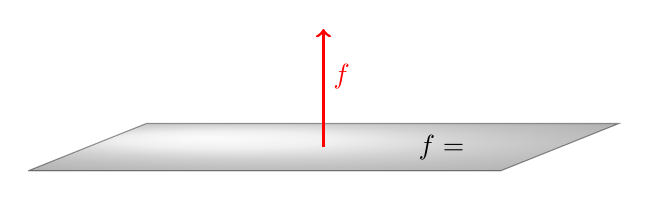
\begin{tikzpicture}[scale=1.5]
  \draw[ball color = gray!40, opacity = 0.4] (0,0) -- (4,0) -- (5,0.4) -- (1,0.4)-- (0,0);
  \draw (3.5,+0.2) node{$f = \cst$};
    \draw[->, red, line width = 1] (2.5, 0.2)-- (2.5, 1.2);
    \draw[red] (2.5, 0.8) node[right]{$\Grad f$};
\end{tikzpicture}
\end{center}
\item Entre deux surfaces $\S_{1}$ et $\S_{2}$ de niveau $f = \cst_{1}$ et $f = \cst_{2}$ avec $\cst_{2} > \cst_{1}$. Pour $\dl$ allant de $\S_{1}$ vers $\S_{2}$, $\d f >0$ donc $\Grad f \ps \dl > 0$. \imp{Le gradient est toujours orienté dans le sens des $f$ croissants.} 
\begin{center}
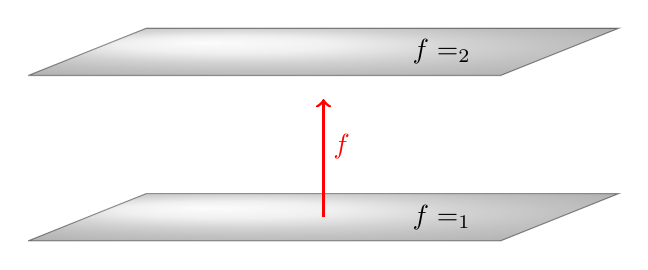
\begin{tikzpicture}[scale=1.5]
  \draw[ball color = gray!40, opacity = 0.4] (0,1.4) -- (4,1.4) -- (5,1.8) -- (1,1.8)-- (0,1.4);
   \draw[ball color = gray!40, opacity = 0.4] (0,0) -- (4,0) -- (5,0.4) -- (1,0.4)-- (0,0);
  \draw (3.5,+0.2) node{$f = \cst_{1}$};
  \draw (3.5,+1.6) node{$f = \cst_{2}$};
    \draw[->, red, line width = 1] (2.5, 0.2)-- (2.5, 1.2);
    \draw[red] (2.5, 0.8) node[right]{$\Grad f$};
\end{tikzpicture}
\end{center}
\end{liste}

\noindent Expression dans différents système de coordonnées :
\begin{liste}
\item En cartésien \eq{\Grad f = \dr{f}{x}\ex + \dr{f}{y}\ey + \dr{f}{z}\ez}
\item En cylindrique \eq{\Grad f = \dr{f}{r}\er + \frac{1}{r} \dr{f}{\theta}\et + \dr{f}{z}\ez}
\item En sphérique \eq{\Grad f = \dr{f}{r}\er + \frac{1}{r} \dr{f}{\theta}\et + \frac{1}{r \sin(\theta)} \dr{f}{\varphi}\ep}
\end{liste}

\parag{Potentiel électrostatique $\rm{V}$}

\noindent Lorsque le travail d'une force $\Vec{f}$ ne dépend pas du chemin suivi, on dit que cette force est conservative est qu'elle dérive d'une énergie potentielle $E_{p}$ telle que le travail élémentaire $\dW$ est :
\eq{\dW = \Vec{f} \ps \dl = - \d E_{p}.}
\noindent C'est à dire que :
\eq{ \Vec{f} = - \Grad{E_{p}} }
\noindent De la même fa\c con, $\E$ étant à \imp{circulation conservative}, il dérive d'un potentiel scalaire. 
\begin{definition}
On appelle \imp{potentiel électrostatique} le potentiel scalaire $V(M)$ (en volt, $\SI{}{V}$) tel que :
\eq{\E = - \Grad V}
\eq{ \textnormal{et} \quad \d \mc{C} = \E \ps \dl = - \d V}
\end{definition}

\begin{remarque}
\begin{liste}
\item Le champ $\E$ s'exprime donc en $\SI{}{V.m^{-1}}$.
\item Comme l'énergie potentielle, le potentielle électrostatique est défini à une constante près.
\end{liste}
\end{remarque}


\noindent Pour une charge ponctuelle, \eq{\vv{E}(M) = \frac{q}{4\pi\varepsilon_0 r^2}\,\vv{e_r} = - \Grad V(M) }
\eq{\dr{V}{r} = - \frac{q}{4\pi\varepsilon_0 r^2}}
\eq{V(r) = \frac{q}{4\pi\varepsilon_0 r} + \cst }
\begin{remarque}
En générale, on fait le choix de prendre un potentiel nul en l'infini ce qui revient à prendre $\cst = 0$.
\eq{\lim_{r \to \infty} V(r) = 0 = \cst}
\end{remarque}

\noindent Pour une distribution discrète de charges ponctuelles $\mc{D} = \{(q_{i}, P_{i})\}_{\mc{D}}$ :
\eq{V(M) = \sum_{i} \frac{q_{i}}{4\pi\varepsilon_0 \nv{P_{i}M} } + \cst }

\noindent Pour des distributions continues :
\begin{liste}
\item linéique $(\mc{L})$ \eq{V(M) = \frac{1}{4\pi\varepsilon_0} \int_{P \in (\mc{L})}  \frac{\lambda(P) \dls(P)}{\nv{PM}} + \cst}
\item surfacique $(\mc{S})$ \eq{V(M) = \frac{1}{4\pi\varepsilon_0} \int_{P \in (\mc{S})}  \frac{\sigma(P) \d \mc{S}(P)}{\nv{PM}} + \cst}
\item volumique $(\mc{V})$ \eq{V(M) = \frac{1}{4\pi\varepsilon_0} \int_{P \in (\mc{V})}  \frac{\rho(P) \d \mc{V}(P)}{\nv{PM}} + \cst}
\end{liste}

\begin{remarque}
En électrocinétique, une tension $U_{\rm{AB}}$ correspond à une différence de potentiel entre les points $\rm{A}$ et $\rm{B}$, $U_{\rm{AB}}=V_{\rm{A}}-V_{\rm{B}}$. Par définition du gradient, la variation du potentiel le long d’un segment infinitésimal $\d \ell$ vaut
\eq{U_{\rm{AB}} = V_{\rm{A}}-V_{\rm{B}} = \int_{\rm{B}}^{\rm{A}} \d V= \int_{\rm{B}}^{\rm{A}} \grad{V}\cdot\vv{\d l}=- \int_{\rm{B}}^{\rm{A}} \vv{E}\cdot\vv{\d l}.}
\end{remarque}
	
\subsection{Énergie potentielle électrostatique}

\parag{Travail de la force électrostatique}

\noindent La force exercée par un champ $\E$ sur une charge $q$ est donné par la partie électrique de la force de Lorentz : \eq{\Vec{f} = q \E}
\noindent Le travail de cette force entre les points $\rm{A}$ et $\rm{B}$ est :
\begin{align*}
W_{\rm{AB}} &= \int_{\rm{A}}^{\rm{B}} \Vec{f} \ps \dl = q  \int_{\rm{A}}^{\rm{B}} \E \ps \dl \\
&= -q  \int_{\rm{A}}^{\rm{B}} \Grad{V} \ps \dl = -q  \int_{\rm{A}}^{\rm{B}} \d V \\
&= q\( V_{\rm{A}} - V_{\rm{B}} \)
\end{align*}

\parag{Energie potentielle d'une charge électrique placée dans un champ électrostatique extérieur}

\eq{\dW = q \E \ps \dl = -q \d V = - \d E_{p}}

\begin{definition}
L'\imp{énergie potentielle} $E_{p}$ exprimée en $\SI{}{J}$ d'une charge $q$ dans un champ électrostatique extérieur créant le potentiel électrostatique $V$ est : \eq{E_{p} = q V + \cst}
\end{definition}

\begin{liste}
\item $W_{\rm{AB}} = - \Delta E_{p} = q \(V_{\rm{A}} - V_{\rm{B}} \)$
\item $\Vec{f} = q \E = - q \Grad V = - \Grad(qV) = -\Grad E_{p}$
\item La champs $\E$ est à circulation conservative et la force électrostatique qui en découle est une force conservative.
\end{liste}
\begin{remarque}
Si un opérateur déplace une charge $q$ dans $E$ de manière réversible (infiniment lentement), il exerce la force : \eq{\Vec{f}_{\rm{op}} = -q \E = q \Grad V = \Grad E_{p}}
\eq{W_{\rm{op}} = \Delta E_{p}}
\end{remarque}

\begin{prop}
L'\imp{énergie potentielle électrostatique} correspond au \imp{travail nécessaire pour construire le système électrique de manière réversible}.
\end{prop}

\begin{exemple}{L'électron-Volt}
L'électron-Volt ($\SI{}{eV}$) est une unité d'énergie. Un électron-Volt est l'énergie cinétique acquise par un électron accéléré depuis le repos sous une différence de potentiel de $\SI{1}{V}$. Déterminer la valeur en Joules de $\SI{1}{eV}$.

\begin{solu}
\begin{center}
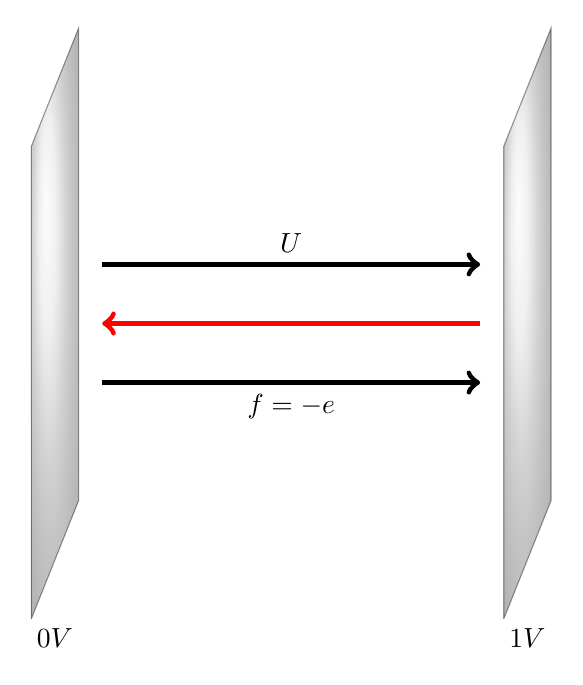
\begin{tikzpicture}[scale=1.5]
   \draw[ball color = gray!40, opacity = 0.4] (0,0) -- (0,4) -- (0.4,5) -- (0.4,1)-- (0,0);
   \draw[ball color = gray!40, opacity = 0.4] (4,0) -- (4,4) -- (4.4,5) -- (4.4,1)-- (4,0);
  \draw (0.2,0) node[below]{$0 \SI{}{V}$};
  \draw (4.2,0) node[below]{$1 \SI{}{V}$};
    \draw[->, red, line width = 2] (3.8, 2.5)-- (0.6, 2.5) node[midway, below]{$\E$};
    \draw[<-, line width = 2] (3.8, 3)-- (0.6, 3) node[midway, above]{$U$};
    \draw[<-, black, line width = 2] (3.8, 2)-- (0.6, 2) node[midway, below]{$\vv{f} = -e \E$};
\end{tikzpicture}
\end{center}

\noindent L'électron n'étant soumise qu'à la force électrostatique conservative, son énergie mécanique $E_{m}$ est constante.
\begin{align*}
E_{m,i} &= E_{m,f} \\
E_{c,i} + E_{p,f} &= E_{c,f} + E_{p,f} \\
\canc{E_{c,i}} + \canc{E_{p,f}} &= E_{c,f} + E_{p,f} 
\end{align*} 
\eq{E_{c,f} = - E_{p,f} = - \( -e \times (V = 1\SI{}{V})\)}
\eq{1 \SI{}{eV} = \SI{1.6e-19}{J}}


\end{solu}

\end{exemple}


\begin{exemple}{Energie potentielle d'interaction entre deux charges}
Quelle est l'énergie potentiel du système suivant ? 
\begin{center}
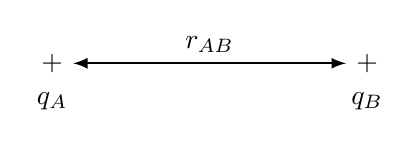
\begin{tikzpicture}[>=latex]
  % Dessin des charges
  \draw[black] (0,0) node[thick,label=below:$q_A$](qA){$+$};
  \draw[black] (4,0) node[thick,label=below:$q_B$](qB){$+$};
  
  % Dessin de la distance entre les deux charges
  \draw[<->,thick] (qA) -- node[above]{$r_{AB}$} (qB);
\end{tikzpicture}
\end{center}

\begin{solu}
\noindent Reformulons la question de la manière suivante : quel est le travail que l'opérateur doit fournir pour construire de manière réversible le système ?

\noindent Initialement, $E_{p} = 0$ et les charges $q_{A}$ et $q_{B}$ sont à l'infini l'une par rapport à l'autre.
\begin{liste}
\item \imp{Etape 1} : On amène $q_{A}$ en $A$ avec $q_{B}$ toujours en l'infini. \eq{W_{\rm{op}} = 0 }
\item \imp{Etape 2} : On amène $q_{B}$ en $B$.
\eq{W_{\rm{op}} = \Delta E_{p} = q_{B} \( V_{A}(B) - \canc{V_{A}(\infty)} \)}
\eq{W_{\rm{op}} = \frac{q_{A} q_{B}}{4 \pi \varepsilon_{0} r_{AB}}}
\end{liste}
\begin{remarque}
Ecrire $E_{p} = \frac{1}{2} \( q_{B} V_{A}(B) + q_{A} V_{B}(A) \)$ permet d'insister sur la symétrie du problème.
\end{remarque}
\end{solu}

\end{exemple}


\section{Topographie du champ électrostatique}

\begin{definition}
\imp{Topographie} : représentation graphique d'un champ en fonction du lieu.
\end{definition}

Dans cette partie, nous expliquons comment représenter un champ électrostatique graphiquement par une carte de champ, et réciproquement comment lire une carte de champ pour en tirer des informations sur le champ électrostatique.

\subsection{Ligne et tube de champ}

\begin{definition}
\imp{Lignes de champ} : courbes tangentes au champ en tout point de l'espace.
\end{definition}

\parag{Lignes de champ créés par une charge ponctuelle}
Le champ électrostatique créé par une charge ponctuelle est de la forme $\Vec{E}(M) = E_r(r) \er$. Par définition, les lignes de champ sont donc radiales (dirigées suivant le vecteur radial $\er$).

Les lignes de champ vérifient les propriétés suivantes :
\begin{liste}
\item Le champ électrostatique $\Vec{E}(M)$ a une norme et une orientation bien défini en un point $M$ donné et ne subit pas de discontinuité (sauf au point où se situe une charge ponctuelle). Ainsi, les lignes de champ sont \important{continues} et deux lignes de champ ne peuvent \important{pas se couper}.
\item Le champ est dirigé vers l’extérieur pour une charge positive. Ainsi, les lignes de champ \imp{sortent} des charges positives et \imp{convergent} vers les charges négativent.
%Les lignes sont de plus \important{orientées selon les potentiels décroissants} (puisque $\vv{E}=-\grad{V}$).
\item Plus les lignes de champ sont resserrées, plus le champ électrostatique est \imp{intense} (ce résultat découle du théorème de Gauss que nous verrons en \Sec{integr}).
\item Les lignes de champ électrostatique ne peuvent \imp{pas être fermées}. Si c'était le cas alors aurait le long de la ligne de champ tous les éléments $\E \ps \dl$ de même signe et non nul et on aurait alors un contour fermé sur lequel la circulation du champ $\E$ serait non nul ce qui n'est pas possible. 
\end{liste}

\noindent On peut préciser le sens du champ $\E$ avec une flèche et son intensité avec la longueur de la flèche.
\begin{liste}
\item Charge ponctuelle positive $+q$ en $O$ : point de divergence des lignes de champs
\begin{center}
\begin{tikzpicture}[scale = 0.5]
% dessiner la charge positive
  \fill[fill=red] (0,0) circle (8pt) node[red,above left]{$+q$}node[above right]{$O$}; % point central de la sphère

  % dessiner les flèches
  \pgfmathsetmacro\raison{0.7}
  \pgfmathsetmacro\offset{0.2}
  \foreach \j in {1,...,5}
      \foreach \i in {1,...,5}
        \draw[->, line width = 1] ({(0.5 + \offset*\i + (2/(1-\raison))*(1-\raison^(\i-1)))*cos(90 + 72*\j)},{(0.5 +\offset*\i + (2/(1-\raison))*(1-\raison^(\i-1)))*sin(90 + 72*\j)}) -- ({(0.5 +\offset*\i + (2/(1-\raison))*(1-\raison^(\i-1)) + 2*\raison^(\i))*cos(90 + 72*\j)}, {(0.5 +\offset*\i + (2/(1-\raison))*(1-\raison^(\i-1)) + 2*\raison^(\i))*sin(90 + 72*\j)});
\end{tikzpicture}
\end{center}
\item Charge ponctuelle négative $-q$ en $O$ : point de convergence des lignes de champs
\begin{center}
\begin{tikzpicture}[scale = 0.5]
  % dessiner la charge positive
  % dessiner la charge positive
  \fill[fill=blue] (0,0) circle (8pt) node[blue,above left]{$-q$}node[above right]{$O$}; % point central de la sphère

  % dessiner les flèches
  \pgfmathsetmacro\raison{0.7}
  \pgfmathsetmacro\offset{0.2}
  \foreach \j in {1,...,5}
      \foreach \i in {1,...,5}
        \draw[<-, line width = 1] ({(0.5 + \offset*\i + (2/(1-\raison))*(1-\raison^(\i-1)))*cos(90 + 72*\j)},{(0.5 +\offset*\i + (2/(1-\raison))*(1-\raison^(\i-1)))*sin(90 + 72*\j)}) -- ({(0.5 +\offset*\i + (2/(1-\raison))*(1-\raison^(\i-1)) + 2*\raison^(\i))*cos(90 + 72*\j)}, {(0.5 +\offset*\i + (2/(1-\raison))*(1-\raison^(\i-1)) + 2*\raison^(\i))*sin(90 + 72*\j)});
\end{tikzpicture}
\end{center}
\end{liste}

\begin{prop}\label{prop:}
Les lignes de champ vérifient, avec $\dl$ le vecteur déplacement élémentaire, l'équation :
\eq{\dl \pv \E = \Vec{0}}
\begin{center}
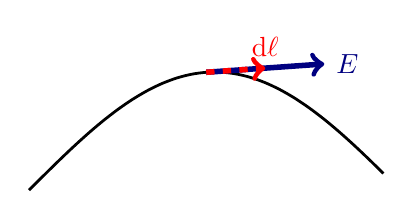
\begin{tikzpicture}[scale=1.5]
  % dessiner la courbe
  \draw[smooth, domain=0:3, line width = 1] plot (\x, {sin(\x r)});

  % choisir un point sur la courbe
  \coordinate (A) at (1.5, {sin(1.5 r)});

  % calculer la pente de la courbe au point A
  \pgfmathsetmacro\slope{cos(1.5 r)}

  % dessiner les vecteurs tangent à la courbe
  \draw[->, thick, blue!50!black, line width = 2] (A) -- ++(1, {\slope}) node[right]{$\Vec{E}$};
  \draw[->, dashed, red, line width = 2] (A) -- ++(0.5, {0.5*\slope}) node[above]{$\mathrm{d}\Vec{\ell}$};
\end{tikzpicture}
\end{center}
\end{prop}
\begin{remarque}
En coordonnées cartésiennes, les lignes de champ ont donc pour équation \eq{\dfrac{\mathrm{d}x}{E_{x}}=\dfrac{\mathrm{d}y}{E_{y}}=\dfrac{\mathrm{d}z}{E_{z}}.}
En coordonnées cylindriques et sphériques on obtient respectivement:
\begin{equation*}
\begin{split}
\dfrac{\mathrm{d}r}{v_{r}}=\dfrac{r\,\mathrm{d}\theta}{v_{\theta}}=\dfrac{\mathrm{d}z}{v_{z}}\qquad\text{et}\qquad \dfrac{\mathrm{d}r}{v_{r}}=\dfrac{r\,\mathrm{d}\theta}{v_{\theta}}=\dfrac{r\sin\theta\,\mathrm{d}\varphi}{v_{\varphi}}.
\end{split}
\end{equation*}
\end{remarque}


\begin{definition}
On appelle aussi \imp{tube de champ} un ensemble de lignes de champ qui s'appuient sur un contour fermé. Lorsqu’un tube de champ s’évase, l’intensité du champ électrostatique diminue ; lorsqu’il se resserre, l’intensité du champ électrostatique augmente.
\begin{center}
\begin{tikzpicture}[scale=0.5]

\draw (0,2) arc (90:-90:0.6 and 2); % section transversale de la sphère
\draw[] (0,2) arc (90:270:0.6 and 2); % section transversale de la sphère opposée

\draw (10,4) arc (90:-90:0.6 and 3); % section transversale de la sphère
\draw[dashed] (10,4) arc (90:270:0.6 and 3); % section transversale de la sphère opposée

\draw[black, thick, postaction={decorate,decoration={markings, mark=at position 0.5 with {\arrow{>}}}}, smooth, tension=0.8] (0,2) to [out=-20,in=160] (10,4) ;
\draw[black, thick, postaction={decorate,decoration={markings, mark=at position 0.5 with {\arrow{>}}}}, smooth, tension=0.8] (0,-2) to [out=40,in=-170] (10,-2) ;
\draw[black, thick, postaction={decorate,decoration={markings, mark=at position 0.5 with {\arrow{>}}}}, smooth, tension=0.8] (0.6,0) to [out=-10,in=-150] (10.6,1) ;
\draw[black, dashed, thick, postaction={decorate,decoration={markings, mark=at position 0.5 with {\arrow{>}}}}, smooth, tension=0.8] (-0.6,0) to [out=15,in=-165] (9.4,1) ;



\end{tikzpicture}
\end{center}
\end{definition}


\subsection{Surface équipotentielle}

\begin{definition}
Une surface \imp{équipotentielle} est une surface $S$ où le potentiel électrostatique est constant, soit
\begin{equation*}
V(M\in S) = \cst.
\end{equation*}
\end{definition}

\noindent Les surfaces équipotentielles ont les propriétés suivantes.
\begin{liste}
\item Le long d’une surface équipotentielle, on a $
 0=\d V=\grad{V}\cdot\dl=-\E\cdot\dl $, soit
$\E\perp\dl$. Ainsi, les surfaces équipotentielles sont \important{orthogonales} aux lignes de champ.
\item La variation du potentiel le long d’une ligne de champ vaut $\d V = -\E\cdot\dl = -E\dl < 0$ avec $E$ la norme du champ. Ainsi, les lignes de champ sont orientées selon les \important{potentiels décroissants}.
\end{liste}

\begin{remarque}
On retrouve les propriétés du gradient.
\end{remarque}

\subsection{Exemples de cartes de champ}

Une \imp{carte de champ} est la représentation graphique d’un ensemble de lignes de champ, éventuellement accompagné de surfaces équipotentielles. Nous représentons quelques cartes de champ produites par une charge ponctuelle (\Fig{1q}) ou deux charges ponctuelles (\Fig{2q}).
 %%%%%%%%%%%%%%%%%%%%%%%%%%%
 \begin{figure}[h!]
\centering
\subfigure[]{\label{fig:1qpos}
\includegraphics[height=0.3\textwidth]{1qpos.pdf}
}
\subfigure[]{\label{fig:1qneg}
\includegraphics[height=0.3\textwidth]{1qneg.pdf}
}
\caption{Lignes de champ (en orange) et équipotentielles (en bleu) du champ électrostatique créé par une charge ponctuelle (a) positive $+q$ et (b) négative $-q$. Les équipotentielles sont toutes séparées d’une même tension $\Delta V$. Comme le champ croît vers le centre, les lignes de champ et les équipotentielles sont plus resserrées.
}
\label{fig:1q}
\end{figure}
%%%%%%%%%%%%%%%%
\begin{figure}[h!]
\centering
\subfigure[]{\label{fig:qpos_equi}
\includegraphics[height=0.3\textwidth]{qpos_equi.pdf}
}
\subfigure[]{\label{fig:qneg_equi}
\includegraphics[height=0.3\textwidth]{qneg_equi.pdf}
}
\subfigure[]{\label{fig:3qneg}
\includegraphics[height=0.3\textwidth]{3qneg.pdf}
}
\caption{Cartes de champ dans un plan $(x,y)$ pour (a) deux charges positives $+q$, (b) deux charges opposées $+q$ et $-q$, et (c) pour une charge $+2q$ et une charge $-q$.}
\label{fig:2q}
\end{figure}
%%%%%%%%%%%%%%%%%%%%%%%%

\begin{exemple}{Lire une carte de champ}
On étudie les distributions de charges des Fig.~\ref{fig:1q} et \ref{fig:2q} dans le repère $(O,\ex,\ey)$. Pour les distribution de la Fig.~\ref{fig:1q}, la charge sera considérée en l'origine et pour la Fig.~\ref{fig:2q} une considérée en $A(-1,0)$ et l'autre en $B(+1,0)$.

\noindent Discuter de l'existence des points de champ nul et dans le cas de leur existence déterminer leur position.

\begin{solu}
\noindent Dans le cas d'une charge ponctuelle, le champ est non nulle en tout point \eq{\frac{q}{4 \pi \varepsilon_{0} r^2} \neq 0 \quad \quad \quad \forall r \in \R_{+}}.
Dans le cas de deux charges, les champs $\E_{A}$ et $\E_{B}$ doivent être colinéaire donc les points de champ nul sont à rechercher sur l'axe $(Ox)$ dans notre cas.
\begin{liste}
\item \imp{Fig.~\ref{fig:qpos_equi}} : En $M(x\in]-1;1[,0)$ : \eq{\E_{A}(M) = \frac{q}{4 \pi \varepsilon_{0} (x+1)^2} \ex }
\eq{\E_{B}(M) = -\frac{q}{4 \pi \varepsilon_{0} (x-1)^2} \ex }
\eq{\E_{\rm{tot}}(M) = \E_{A}(M) + \E_{B}(M) }
\eq{\E_{\rm{tot}}(M) = 0 \quad \quad \quad \Leftrightarrow \quad \quad \quad x=0 }
\item \imp{Fig.~\ref{fig:qneg_equi}} et \imp{Fig.~\ref{fig:3qneg}} : Pas de solution.
\end{liste}
\end{solu}

\end{exemple}

\FloatBarrier

\section{Symétries et invariances du champ électrostatique}
\label{sec:topographie_symétrie_invariances}

Dans le cas général, le champ électrostatique possède trois composantes qui chacune peuvent dépendre de trois coordonnées spatiales ; par exemple en coordonnées cartésiennes
\begin{equation*}
\vv{E}=E_x(x,y,z)\,\vv{e_x}+E_y(x,y,z)\,\vv{e_y}+E_z(x,y,z)\,\vv{e_z}.
\end{equation*}
On souhaiterait pouvoir prédire si le champ ne dépend pas de certaines variables (analyse des invariances du champ) ou est nul selon certaines composantes (analyse des symétries du champ). L’intérêt de cette approche est double.
\begin{liste}
\item D’un point de vue conceptuel, elle permet d’obtenir des informations sans pour autant connaître les lois de l’électrostatique (que nous verrons en \Sec{lois}).
\item D’un point de vue pratique, elle permet d’économiser beaucoup de calculs lorsque la distribution de charge possède de nombreuses symétries.
\end{liste}
 L’idée derrière cette analyse vient d’un principe très général, le \imp{principe de Curie} : « Les invariances et symétries des causes se retrouvent dans les effets ».
En électrostatique, les causes sont la distribution de charge, et les effets le champ ou le potentiel électrostatique. 

\subsection{Invariances du champ et du potentiel}


On appelle \imp{invariance} d'une distribution de charge une transformation de translation ou de rotation qui laisse la distribution inchangée. L'étude des invariances permet de limiter le nombre de \important{coordonnées} dont dépendent le champ et le potentiel électrostatiques. Le principe de Curie permet d'affirmer que $\vv{E}$ et $V$ possède les mêmes invariances que la distribution de charge (par exemple la densité volumique de charge $\rho$) qui leur donne naissance.

\begin{prop}[Principe de Curie]\label{prop:curie}
Les invariants d’une distribution de sources laissent invariant la distribution des effets. Les mêmes causes produisent les mêmes effets et toute transformation laissant invariant les causes laisse invariant les effets.\end{prop}
\begin{remarque}
  Ce principe très général doit être pris avec précaution. Ce sont \emph{in fine} les équations fondamentales de la physique qui dictent les invariances et symétries des champ. En particulier, ce principe ne s'applique plus tel quel en régime variable, ou le champ magnétique peut aussi contrôler les symétries de $\Vec{E}$.
\end{remarque}
% Bien souvent, une invariance permet d’affirmer que $\Vec{E}$ et $V$ ne dépendent que d'une variable, par exemple $x$ ou $r$.
%
Voici les invariances usuelles d'une distribution de charges.
\begin{liste}
\item Invariance par \imp{translation} selon un axe $(Ox)$ : $\rho$ ne dépend pas de $x$.
\item Invariance par \imp{rotation} d'angle $\theta$ autour d'un axe $(Oz)$ : $\rho$ ne dépend pas de $\theta$.
\item Invariance par translation selon et rotation autour de $(Oz)$ (symétrie cylindrique) : \\$\rho(r,\theta,z)=\rho(r)$.
\item Invariance par rotation autour de tout axe passant par l’origine $O$  (symétrie sphérique) : \\ $\rho(r,\theta,\varphi)=\rho(r)$.
\end{liste}
Les invariances précédentes de la distribution de charges se retrouvent d'après le principe de Curie dans les invariances de $\vv{E}$ et de $V$.

\begin{remarque}
Dans le premier cas ci-dessus, les composantes de $\vv{E}$, à savoir $E_{x}$, $E_y$ et $E_z$, ne dépendent pas de $x$. Dans le dernier cas, où la distribution de charges possède une symétrie sphérique, alors cette invariance permet d'écrire que $\vv{E}(r,\theta,\varphi)=\vv{E}(r)$.
\end{remarque}

\begin{exemple}{Fil infini uniformément chargé}
Considérons une distribution linéique uniforme de charges assimilée à un fil infini selon $(Oz)$. On note $\lambda(z)$ la densité linéique de charge et on utilise les coordonnées cylindriques. Le fil étant infini et la distribution uniforme, la distribution de charge est invariante par translation selon $(Oz)$. On a alors $\lambda(\canc{z}) = \lambda$.
Ainsi, $\vv{E}$ et~$V$ ne dépendent pas de la coordonnée $z$, soit
\begin{equation*}
\vv{E}=E_r(r,\theta,\canc{z})\er+E_\theta(r,\theta,\canc{z})\et+E_z(r,\theta,\canc{z})\ez, \qquad \text{et} \qquad V(r,\theta,\canc{z}).
\end{equation*}
De plus, la distribution de charges est invariante par rotation d'angle $\theta$ autour de l'axe $(Oz)$, et donc
\begin{equation*}
\vv{E}=E_r(r,\canc{\theta})\vv{e_r}+E_\theta(r,\canc{\theta})\vv{e_\theta}+E_z(r,\canc{\theta})\vv{e_z}, \qquad \text{et} \qquad V(r,\canc{\theta}).
\end{equation*}
En conclusion, $\Vec{E}(r)$ et $V(r)$ ne dépendent que de $r$.

\end{exemple}

\begin{remarque}
Dans le cas général, le principe de Curie n'est vrai que en moyenne. En effet, on peut prendre deux exemples où il faut moyenner pour ne pas mettre en défaut le principe de Curie :
\begin{liste}
\item Lorsqu'une bille se situe en haut d'une barrière de potentiel à une dimension, elle se trouve dans un état métastable. Elle peut tomber soit à gauche ou soit à droite quand on la lâche en haut.
\item Lorsqu'une tige rigide d'une certaine longueur est fixée dans un mur, si on appuie sur la tige dans son axe alors la tige va flamber. Elle peut flamber dans n'importe quelle direction de l'espace, c'est-à-dire sous n'importe quel angle entre 0 et 2$\pi$.
\end{liste}
Dans ce deux cas on a une symétrie du système et si on fait une expérience le système va "choisir" une direction et donc briser cette symétrie. Cependant si on répète un grand nombre de fois l’expérience et qu’on trace la distribution de probabilité alors celle-ci va posséder les mêmes symétries que le système. Le principe de Curie est alors vérifié.
Une autre manière de le dire est qu’il faut retrouver le principe de Curie sur l’ensemble des solutions et non sur une solution particulière.
\end{remarque}


\subsection{Le champ électrique est un vrai vecteur}
Nous distinguons en physique les vrais vecteurs et les pseudo-vecteurs. Un vrai vecteur est un vecteur qui ne dépend pas de la règle d'orientation de l'espace (règle de la main droite). C'est par exemple le cas du vecteur position $\vv{r}$ et de ses dérivées (vitesse $\vv{v}$, accélération $\vv{a}$ et donc force $\vv{F}$ d'après la loi de Newton). D'après la loi de Coulomb, on peut en déduire que le champ électrique $\vv{E}$ est un vrai vecteur.

Mais il existe aussi des pseudo-vecteurs, dont l'orientation dépend de celle choisie pour orienter l'espace. C'est le cas de toutes les grandeurs vectorielles définies comme produits vectoriels de vrais vecteurs, par exemple le moment d'une force $\vv{r}\pv\vv{F}$ est un pseudo-vecteur.
\begin{remarque}
De façon générale, prendre un produit vectoriel revient à changer un vrai vecteur en pseudo-vecteur et réciproquement. Schématiquement,
\begin{equation*}
\begin{split}
&\text{vrai}\pv\text{vrai}=\text{pseudo}\\
&\text{vrai}\pv\text{pseudo}=\text{vrai}\\
&\text{pseudo}\pv\text{pseudo}=\text{pseudo}.
\end{split}
\end{equation*}
\end{remarque}
L'exemple que nous rencontrerons bientôt est celui du champ magnétique $\vv{B}$. En effet, d'après l'expression de la force magnétique de Lorentz $\vv{F}=q\vv{v}\pv\vv{B}$. Or $\vv{F}$ et $\vv{v}$ sont des vrais vecteurs, d'où on déduit que $\vv{B}$ est un pseudo-vecteur.

%\clearpage
\subsection{Symétries du champ}

%%%%%%%%%%%%%%%%%%%
\begin{figure}[H]
\centering
\includegraphics[width=0.7\textwidth]{sym_antisym.pdf}
\caption{Le champ électrostatique $\vec{E}$ appartient aux plans de symétrie de la distribution de charges, et est orthogonal à un plan d'antisymétrie de la distribution de charges.}
\label{fig:sym_antisym}
\end{figure}
%%%%%%%%%%%%%%%%%%%

%%%%%%%%%%%%%%
\begin{figure}[H]
\centering
\includegraphics[width=0.35\textwidth]{fil_infini.pdf}
\caption{Plans de symétrie (en vert) de la distribution de charges d'un fil infini dirigé selon $\vec{e}_z$. Le champ électrostatique appartient à l'intersection des plans, et est donc dirigé selon $\vec{e}_r$.}
\label{fig:fil_infini}
\end{figure}
%%%%%%%%%%%%%%%%%%%

On appelle \imp{symétrie} d’une distribution de charge toute transformation miroir qui transforme la distribution de charge en la distribution identique (plan de symétrie) ou la distribution opposée (plan d’antisymétrie).
%
%L'étude des symétries permet de limiter le nombre de \important{composantes} dont dépendent les champ. Dans le meilleur des cas (si les symétries de la distribution de charges sont suffisantes), on peut alors déterminer la direction du vecteur $\vv{E}$.
%On cherche à repérer des plans de symétrie ou d'antisymétrie de la distribution de charges.
Le champ $\vv{E}$ étant un vecteur au sens strict du terme (il ne dépend pas de l’orientation de l’espace), il possède les propriétés suivantes expliquées sur la Fig.~\ref{fig:sym_antisym}.

\begin{liste}
\item Il appartient à tout plan de symétrie $\Pi_{\rm{S}}(M)$ de la distribution de charges contenant le point courant $M$, soit $\Vec{E}(M) \in \Pi_{\rm{S}}(M)$. Pour fixer la direction, il est alors nécessaire que le système possède deux plans de symétrie qui s’intersectent.
\item Il est orthogonal à tout plan d'antisymétrie $\Pi_{\rm{AS}}(M)$ de la distribution de charges contenant le point courant $M$, soit $\Vec{E}(M) \perp \Pi_{\rm{AS}}(M)$. Pour fixer la direction, il ne faut qu’un plan d’antisymétrie.
\end{liste}

\begin{remarque}
Soit $\mc{D}$ une distribution de charges. Soit $\Pi_{\rm{S}}$ un plan de symétrie de la distribution de charges. Ainsi, pour tout $M \in D$, si $M'$ est le symétrique du point $M$ par rapport au plan $\Pi_{\rm{S}}$, qu'on notera $M' = \rm{sym}_{\Pi_{\rm{S}}}(M)$, alors on a nécessairement $\rho(M) = \rho(M')$. De même, si $\Pi_{\rm{AS}}$ est un plan d'antisymétrie de la distribution de charge, alors si $M' = \rm{sym}_{\Pi_{\rm{AS}}}(M)$, alors on a $\rho(M) = -\rho(M')$.

Si on se place dans le cas où la distribution possède une symétrie $\Pi_{\rm{S}}$, soit $M$ et $M'$ deux points symétriques l'un par rapport à l'autre par $\Pi_{\rm{S}}$, et soit $P$ un point de $\mc{D}$. Calculons alors le champ créé au point $M$ par la distribution $\mc{D}$.
\eq{\E(M) = \int_\mc{D} \d \E_{P}(M) = \int_\mc{D} \frac{\rho(P)}{4\pi\epsilon_0} \frac{\Vec{PM}}{\nv{PM}^3} \d\mc{V}(P)}
On peut alors calculer le champ créé au point $M$ par les points $P$ et $P'$ symétriques par rapport au plan $\Pi_{\rm{S}}$. Par superposition on a :
\eq{\d\E_{P,P'}(M)=\frac{\d\mc{V}(M)}{4\pi\varepsilon_{0}}\(\frac{\rho(P)}{\nv{PM}^3} \Vec{PM}+\frac{\rho(P')}{\nv{P'M}^3} \Vec{P'M}\)}
On peut ensuite calculer le champ créé au point M' par les mêmes points P et P'. On exprime alors $\Vec{PM'}$ et $\Vec{P'M'}$ comme les symétriques de $\Vec{P'M}$ et $\Vec{PM}$. On remarque également par symétrie que les distances $\nv{PM'}$ et $\nv{P'M}$ sont égales ainsi que les distances $\nv{P'M'}$ et $\nv{PM}$. Enfin par hypothèse on a $\rho(P') = \rho(P)$.
\begin{align*}
\d\E_{P,P'}(M') &= \frac{\d\mc{V}(M')}{4\pi\varepsilon_{0}}\(\frac{\rho(P)}{\nv{PM'}^3} \Vec{PM'}+\frac{\rho(P')}{\nv{P'M'}^3} \Vec{P'M'}\) \\
&= \frac{\d\mc{V}(M')}{4\pi\varepsilon_{0}}\(\frac{\rho(P)}{\nv{P'M}^3} \rm{sym}_{\Pi_{\rm{S}}}(\Vec{P'M})+\frac{\rho(P')}{\nv{PM}^3} \rm{sym}_{\Pi_{\rm{S}}}(\Vec{PM})\) \\
&= \frac{\d\mc{V}(M')}{4\pi\varepsilon_{0}}\(\frac{\rho(P')}{\nv{P'M}^3} \rm{sym}_{\Pi_{\rm{S}}}(\Vec{P'M})+\frac{\rho(P)}{\nv{PM}^3} \rm{sym}_{\Pi_{\rm{S}}}(\Vec{PM})\) \\
&= \rm{sym}_{\Pi_{\rm{S}}}(\d\E_{P,P'}(M))
\end{align*}
Ainsi chaque champ élémentaire créé au point $M'$ est symétrique par rapport au plan $\Pi_{\rm{S}}$ au champ élémentaire créé au point $M$. Et par linéarité de l’intégrale on a : \eq{\E(M') = \rm{sym}_{\Pi_{\rm{S}}}(\E(M')).}
La conséquence de cette égalité est que si $M \in \Pi_{\rm{S}}$, alors on applique le résultat précédent avec $M = M'$, et donc on a $E(M) = \rm{sym}_{\Pi_{\rm{S}}}(E(M))$. Ceci a pour conséquence que dans ce cas, on a $E_{\perp}(M) = 0$.

De la même manière, on peut montrer que si on a un plan d’antisymétrie $\Pi_{\rm{AS}}$ de la distribution de charge et $M \in \Pi_{\rm{AS}}$, alors on trouve que $E(M) \perp \Pi_{\rm{AS}}$.

\end{remarque}

\noindent Ainsi les symétries du problème peut permettre de fixer la direction du champ E (ou d’éliminer une composante) en certains points de l’espace.

\begin{liste}
\item Dans l'étude des symétries, le plan de symétrie doit contenir le point $M$ où l'on cherche à calculer le champ $\E$.
\item On commencera toujours un problème par l'étude des :
\begin{enumerate}
\item Invariances (qui donnent les variables dont dépend $\E(M)$
\item Symétries (qui donnent la direction du champ $\E(M)$
\end{enumerate}
\end{liste}

\section{Flux du champ électrostatique - Théorème de Gauss}
\label{sec:Gauss}
A priori, il est possible de calculer le champ $\vv{E}$ et le potentiel $V$ à partir de la seule loi de Coulomb, en utilisant les expressions intégrales Éq.~\eqref{eq:champE_distrib_continue}. Le problème est que le calcul direct en utilisant ces équations est difficile à la main ! Il est donc préférable d'utiliser les lois de l’électrostatique qui portent sur le champ $\Vec{E}$ ou le potentiel $V$, surtout lorsque la distribution de charges possède des symétries. Les lois de l’électrostatique peuvent se formuler de manière locale (avec des opérateurs vectoriels) ou intégrale (avec des flux ou des circulations).

\subsection{Flux d'un champ $\E$}

\noindent Soit un champ de vecteur $\E$ prenant la valeur $\E(M)$ en un point $M$ de la surface $(\mc{S})$. Soit $\d \Vec{\mc{S}}(M)$ le vecteur surface élémentaire au point $M$ porté par le vecteur unitaire ${n}_{M}$ orthogonal à $(\mc{S})$ en $M$.
\begin{center}
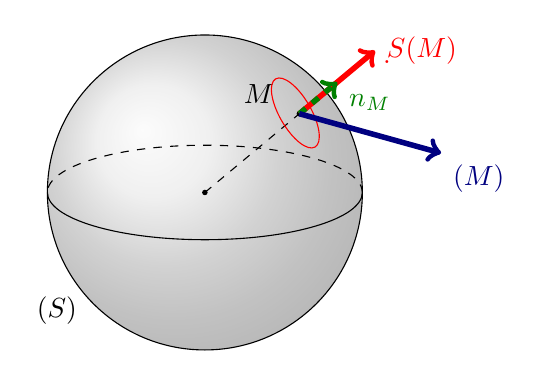
\begin{tikzpicture}
  \shade[ball color = gray!40, opacity = 0.4] (0,0) circle (2cm); % couleur de la sphère et transparence
  \draw (0,0) circle (2cm); % contour de la sphère
  \draw (-2,0) arc (180:360:2 and 0.6); % section transversale de la sphère
  \draw[dashed] (2,0) arc (0:180:2 and 0.6); % section transversale de la sphère opposée
  \fill[fill=black] (0,0) circle (1pt); % point central de la sphère
  \draw[dashed] (0,0 ) -- (1.2,1.0); % rayon de la sphère
  \draw (1.0, 1.0) node[above left]{$M$};
  \fill[fill=black] (1.2,1.0) circle (1pt);
   \rotatebox{30}{\draw[red] (1.5,0.3) ellipse (0.2cm and 0.5cm);}; % ellipse rouge inclinée de 30 degrés
   \draw[red,->, line width = 2] (1.2,1.0) -- (1.8 * 1.2,1.8 * 1.0) node[right]{$\d \Vec{\mc{S}}(M)$}; % vecteur rouge partant de (1.2,1.0)
   \draw[green!50!black,->, line width = 2, dashed] (1.2,1.0) -- (1.4 * 1.2,1.4 * 1.0) node[below right]{$\Vec{n}_{M}$} ;
    \draw[blue!50!black,->, line width = 2] (1.2,1.0) -- (3,0.5) node[below right]{$\E(M)$};
    \draw (-1.5,-1.5) node[left]{$(\mc{S})$};
\end{tikzpicture}
\end{center}

\begin{definition}
Le \imp{flux élémentaire du champ $\E$} à travers la \imp{surface élémentaire}  $\d \Vec{\mc{S}}(M)$ est : \eq{\d \phi_{M} = \E(M) \ps \d \Vec{\mc{S}}(M) = \E(M) \ps \d S(M) \Vec{n}_{M} }
Le flux total de $\E$ à travers $(\mc{S})$ est : \eq{\phi_{(\mc{S})} = \int_{M \in (\mc{S})}  \E(M) \ps \d \Vec{\mc{S}}(M)}
Le flux du champ électrostatique est exprimé en $\SI{}{V . m}$.
\end{definition}

\begin{exemple}{Calcul d'un flux}
Considérons un champ de vitesse uniforme $\Vec{v}$. Ce champ de vitesse représente la vitesse des gouttes de pluie tombant dans un saut. Calculer le débit volumique d'eau de pluie entrant dans le saut.
\begin{center}
\begin{tikzpicture}
	\draw (-2,0) arc (180:360:2 and 0.6); % section transversale de la sphère
	\draw (2,0) arc (0:180:2 and 0.6); % section transversale de la sphère opposée
	\pattern[pattern=north east lines, pattern color=gray] (-2,0) arc (180:360:2 and 0.6) -- (2,0) arc (0:180:2 and 0.6)node[left]{$\mc{S}$} -- cycle;
	% dessiner le vecteur S
\draw[->, line width = 1] (0,0) -- (0,-1) node[left]{$\d \Vec{\mc{S}}$};

% dessiner le vecteur v
\draw[blue!50!black, ->, line width = 1] (0,0) -- (1/3,-1) node[blue!50!black,right]{$\Vec{v}$};

% déterminer les coordonnées pour le point d'intersection des deux vecteurs
\coordinate (O) at (0,0);
\coordinate (S) at (0,-1);
\coordinate (V) at (1/3,-1);

% dessiner l'arc pour l'angle theta
\draw[red, line width = 1] (0,-0.8) arc (-90:-71:0.8) node[midway,above right]{$\theta$};

	\draw (-3,3) arc (180:360:2 and 0.6); % section transversale de la sphère
	\draw (1,3) arc (0:180:2 and 0.6); % section transversale de la sphère opposée
	\draw (-1.5,-2) arc (180:360:1.5 and 0.6); % section transversale de la sphère
	\draw (-1.5,-2)--(-2,0);
	\draw (1.5,-2)--(2,0);
	
	\foreach \j in {1,...,5}
		\draw[blue!50!black, ->, line width = 1] ({-3+(6/10)*(\j+1)},2) -- ({1/3 -3+(6/10)*(\j+1)} ,1);
	\draw (1.5,1.5) node[blue!50!black,right]{$\Vec{v}$};
	\draw[dashed] (-3,3)--(-2,0);
	\draw (-2.5,1.5)node[left]{$\nv{v} \d t$};
	\draw[dashed] (1,3)--(2,0);
\end{tikzpicture}
\end{center}
\begin{solu}
Soit $D_{V}$ le débit volumique. Notons $\d V$ la variation de volume d'eau de pluie à l'intérieur du saut pendant le temps $\d t$. \eq{D_{V} = \dd{V}{t}.}
L'eau entrant dans le saut ne peut se faire que par le haut et l'eau entrant par la surface $\mc{S}$ au cours du temps $\d t$ est celle contenue dans le cylindre incliné de volume : \eq{\d V = \nv{v} \d t \mc{S} \cos{\theta}.}
Ainsi le débit volumique est égale au flux du champ $\Vec{v}$ à travers la surface $\mc{S}$ : \eq{D_{V} = \nv{v} \mc{S} \cos{\theta}.}
\end{solu}

\end{exemple}

\subsection{Théorème de Gauss}

\begin{theorem}[Théorème de Gauss]

Le flux du champ électrostatique $\E$ à travers une surface fermée $(\Sigma)$ est égale à la charge intérieur à cette surface divisée par $\varepsilon_{0}$.
\eq{\oiint_{(\Sigma)} \E \ps \d \Vec{\mc{S}} = \frac{Q_{\rm{int}}}{\varepsilon_{0}} }
On rappelle que la convention est d'orienté le vecteur surface infinitésimal $\d \Vec{\mc{S}}$ vers l'extérieur de la surface.
\end{theorem}

\begin{remarque}
\begin{liste}
\item Le champ électrostatique est à circulation conservative mais il n'est à priori par à flux conservatif.
\item Même si $Q_{\rm{int}}$ ne prend en compte que les charges intérieures à $(\Sigma)$, le champ $\E$ considéré est bien celui créé par toutes les charges intérieures et extérieurs.
\end{liste}
\end{remarque}

\begin{exemple}{Vérification avec le cas une charge ponctuelle}

Montrer que le théorème de Gauss est bien vérifié dans le cas d'une charge ponctuelle $q$ et pour une surface de Gauss fermée $(\Sigma)$ sphérique centrée sur la charge ponctuelle.

\begin{center}
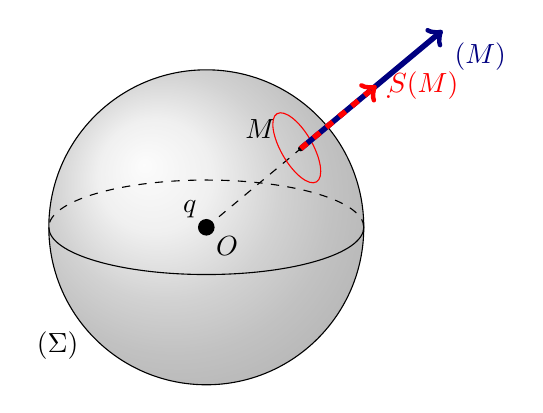
\begin{tikzpicture}
  \shade[ball color = gray!40, opacity = 0.4] (0,0) circle (2cm); % couleur de la sphère et transparence
  \draw (0,0) circle (2cm); % contour de la sphère
  \draw (-2,0) arc (180:360:2 and 0.6); % section transversale de la sphère
  \draw[dashed] (2,0) arc (0:180:2 and 0.6); % section transversale de la sphère opposée
  \fill[fill=black] (0,0) circle (3pt) node[above left]{$q$}node[below right]{$O$}; % point central de la sphère
  \draw[dashed] (0,0 ) -- (1.2,1.0); % rayon de la sphère
  \draw (1.0, 1.0) node[above left]{$M$};
  \fill[fill=black] (1.2,1.0) circle (1pt);
   \rotatebox{30}{\draw[red] (1.5,0.3) ellipse (0.2cm and 0.5cm);}; % ellipse rouge inclinée de 30 degrés
    \draw[blue!50!black,->, line width = 2] (1.2,1.0) -- (2.5 * 1.2,2.5 * 1.0) node[below right]{$\E(M)$};

   \draw[red,->, line width = 2, dashed] (1.2,1.0) -- (1.8 * 1.2,1.8 * 1.0) node[right]{$\d \Vec{\mc{S}}(M)$}; % vecteur rouge partant de (1.2,1.0)

       \draw (-1.5,-1.5) node[left]{$(\Sigma)$};
\end{tikzpicture}
\end{center}

\begin{solu}
Le champ électrostatique en tout point $M$ est \eq{\E(M) = \frac{q}{4\pi \varepsilon r^2} \er.}
L'élément infinitésimale de surface en coordonnée sphérique est \eq{\d \Vec{\mc{S}} = r^2 \sin{\theta} \d\theta \d\varphi \er.}
Donc le flux du champ $\E$ à travers une surface sphérique de rayon $r$ centrée en la charge ponctuelle $q$ prise pour origine du repère est 
\eq{\phi = \oiint_{(\Sigma)} \E \ps \d \Vec{\mc{S}} = \oiint_{(\Sigma)}\frac{q}{4\pi \varepsilon r^2}r^2 \sin{\theta} \d\theta \d\varphi = \frac{q}{\varepsilon_{0}}}
\end{solu}

\end{exemple}

\begin{prop}
Le flux est constant à travers toutes sections d'un tube de champ.
Ainsi, plus la section du tube est étroite et plus le champ est intense.
\end{prop}
\begin{center}
\begin{tikzpicture}[scale=0.5]

\draw (0,2) arc (90:-90:0.6 and 2); % section transversale de la sphère
\draw[] (0,2) arc (90:270:0.6 and 2); % section transversale de la sphère opposée

\draw (10,4) arc (90:-90:0.6 and 3); % section transversale de la sphère
\draw[dashed] (10,4) arc (90:270:0.6 and 3); % section transversale de la sphère opposée

\draw[black, thick, postaction={decorate,decoration={markings, mark=at position 0.5 with {\arrow{>}}}}, smooth, tension=0.8] (0,2) to [out=-20,in=160] (10,4) ;
\draw[black, thick, postaction={decorate,decoration={markings, mark=at position 0.5 with {\arrow{>}}}}, smooth, tension=0.8] (0,-2) to [out=40,in=-170] (10,-2) ;
\draw[black, thick, postaction={decorate,decoration={markings, mark=at position 0.5 with {\arrow{>}}}}, smooth, tension=0.8] (0.6,0) to [out=-10,in=-150] (10.6,1) ;
\draw[black, dashed, thick, postaction={decorate,decoration={markings, mark=at position 0.5 with {\arrow{>}}}}, smooth, tension=0.8] (-0.6,0) to [out=15,in=-165] (9.4,1) ;

\draw[red,->, line width = 1] (10,1) -- (12,1) node[right]{$\d \Vec{\mc{S}}_{2}$};

\draw[red,->, line width = 1, dashed] (0,0) -- (2,0) node[right]{$\d \Vec{\mc{S}}_{1}$};

\draw[green!50!black,->, line width = 1] (6,3.5) -- ({6+2*cos(120)},{3.5+2*sin(120)}) node[right]{$\d \Vec{\mc{S}}_{\rm{lat}}$};


\end{tikzpicture}
\end{center}

\begin{remarque}
A l'intérieur du tube de champ il n'y a pas de charge car pas de point de convergence ou de divergence des lignes de champ.
L'application du théorème de Gauss donne donc
\begin{align*}
\phi = \oiint_{(\Sigma) = (\mc{S}_{1}) \cup (\mc{S}_{2}) \cup (\mc{S}_{\rm{lat}})} \E \ps \d \Vec{\mc{S}} = -\phi_{1} + \phi_{2} + \phi_{\rm{lat}} = 0
\end{align*}
Or $\phi_{\rm{lat}} = 0$ car $\d \Vec{\mc{S}}_{\rm{lat}} \perp \E$ donc \eq{\phi_{1} = \phi_{2}}
\end{remarque}

\begin{prop}
Le potentiel électrostatique ne peut pas atteindre d'extremum en un point de l'espace vide de charge.
\end{prop}

\begin{liste}
\item Un maximum de potentiel est un point de divergence des lignes de champ. On peut alors trouver une surface fermée suffisamment proche de sorte à ce que les lignes de champ traversant la surface le fassent toutes dans le sens intérieur vers extérieur ce qui signifie que le flux du champ $\E$ est en tout point de la surface positif. \eq{\d \phi > 0 \quad \qdonc \quad \frac{Q_{\rm{int}}}{\varepsilon_{0}}> 0}
Il y a donc forcément une charge au point $M$, maximum de potentiel électrostatique, et cette charge est positive.
\begin{center}
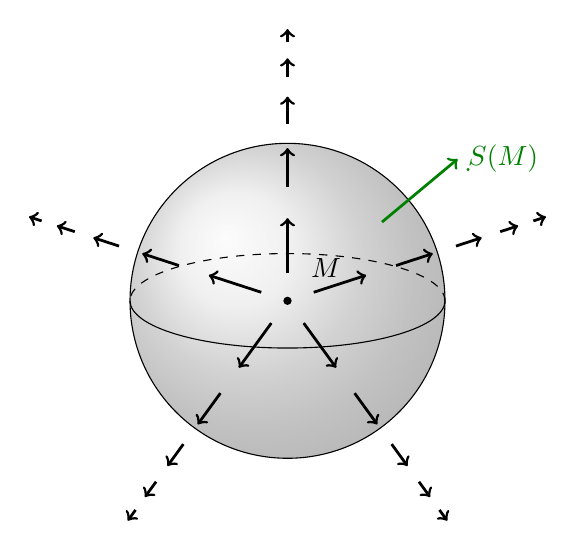
\begin{tikzpicture}[scale = 0.5]
 \shade[ball color = gray!40, opacity = 0.4] (0,0) circle (4cm); % couleur de la sphère et transparence
  \fill[fill=black] (0,0) circle (3pt) node[above right=5pt]{$M$};% point central de la sphère
  \draw (0,0) circle (4cm); % contour de la sphère
  \draw (-4,0) arc (180:360:4 and 1.2); % section transversale de la sphère
  \draw[dashed] (4,0) arc (0:180:4 and 1.2); % section transversale de la sphère opposée
  
  \draw[green!50!black,->, line width = 1] (2 * 1.2, 2 * 1.0) -- (2 * 1.8 * 1.2, 2 * 1.8 * 1.0) node[right]{$\d \Vec{\mc{S}}(M)$}; % vecteur rouge partant de (1.2,1.0)

  % dessiner les flèches
  \pgfmathsetmacro\raison{0.7}
  \pgfmathsetmacro\offset{0.2}
  \foreach \j in {1,...,5}
      \foreach \i in {1,...,5}
        \draw[->, line width = 1] ({(0.5 + \offset*\i + (2/(1-\raison))*(1-\raison^(\i-1)))*cos(90 + 72*\j)},{(0.5 +\offset*\i + (2/(1-\raison))*(1-\raison^(\i-1)))*sin(90 + 72*\j)}) -- ({(0.5 +\offset*\i + (2/(1-\raison))*(1-\raison^(\i-1)) + 2*\raison^(\i))*cos(90 + 72*\j)}, {(0.5 +\offset*\i + (2/(1-\raison))*(1-\raison^(\i-1)) + 2*\raison^(\i))*sin(90 + 72*\j)});
\end{tikzpicture}
\end{center}

\item Un minimum de potentiel est un point de convergence des lignes de champ. On peut alors trouver une surface fermée suffisamment proche de sorte à ce que les lignes de champ traversant la surface le fassent toutes dans le sens extérieur vers intérieur ce qui signifie que le flux du champ $\E$ est en tout point de la surface négatif. \eq{\d \phi < 0 \quad \qdonc \quad \frac{Q_{\rm{int}}}{\varepsilon_{0}}< 0}
Il y a donc forcément une charge au point $M$, minimum de potentiel électrostatique, et cette charge est négative.
\begin{center}
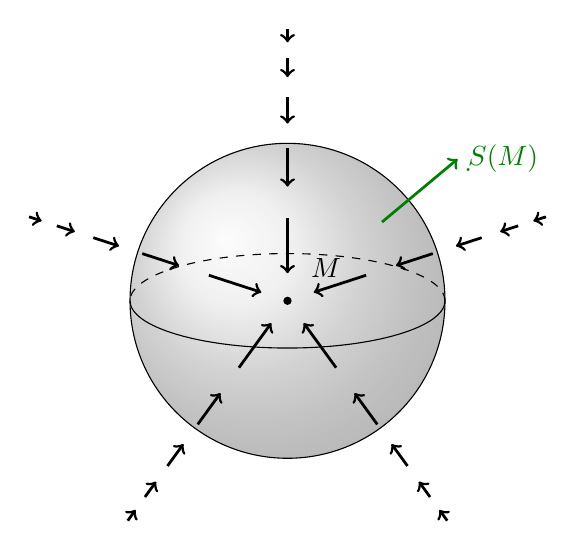
\begin{tikzpicture}[scale = 0.5]
 \shade[ball color = gray!40, opacity = 0.4] (0,0) circle (4cm); % couleur de la sphère et transparence
   \fill[fill=black] (0,0) circle (3pt) node[above right=5pt]{$M$};% point central de la sphère
  \draw (0,0) circle (4cm); % contour de la sphère
  \draw (-4,0) arc (180:360:4 and 1.2); % section transversale de la sphère
  \draw[dashed] (4,0) arc (0:180:4 and 1.2); % section transversale de la sphère opposée
  
  \draw[green!50!black,->, line width = 1] (2 * 1.2, 2 * 1.0) -- (2 * 1.8 * 1.2, 2 * 1.8 * 1.0) node[right]{$\d \Vec{\mc{S}}(M)$}; % vecteur rouge partant de (1.2,1.0)

  % dessiner les flèches
  \pgfmathsetmacro\raison{0.7}
  \pgfmathsetmacro\offset{0.2}
  \foreach \j in {1,...,5}
      \foreach \i in {1,...,5}
        \draw[<-, line width = 1] ({(0.5 + \offset*\i + (2/(1-\raison))*(1-\raison^(\i-1)))*cos(90 + 72*\j)},{(0.5 +\offset*\i + (2/(1-\raison))*(1-\raison^(\i-1)))*sin(90 + 72*\j)}) -- ({(0.5 +\offset*\i + (2/(1-\raison))*(1-\raison^(\i-1)) + 2*\raison^(\i))*cos(90 + 72*\j)}, {(0.5 +\offset*\i + (2/(1-\raison))*(1-\raison^(\i-1)) + 2*\raison^(\i))*sin(90 + 72*\j)});
\end{tikzpicture}
\end{center}
\end{liste}

\noindent Le théorème de Gauss est un outils essentiel pour déterminer le champ $\E$ dans le cas de distribution de charge à haute symétrie.

\subsection{Applications du théorème de Gauss pour le calcul du champ $\E$}

\parag{Méthode}

\begin{enum}
    \item Etude des invariances et des symétries de la distribution de charge qui donnent respectivement les variables dont dépend $\nv{E}$ et la direction de $\E$.
    \item Choix d'une surface de Gauss $(\Sigma)$, celle-ci doit être :
    \begin{liste}
    \item Fermée
    \item Passant par le point $M$ où l'on veut calculer le champ $\E$
    \item Telle que $\E(M)$ soit orthogonale à la surface en tout point, \ie colinéaire à $\d \Vec{\mc{S}}$ de sorte que $\E \ps \d \Vec{\mc{S}} = E \d S$
    \item Telle que $\nv{E}$ soit la même en tout point de la surface de sorte que $\iint E \d S = E \iint \d S$
    
    Idéalement, il faut prendre une \imp{équipotentielle}.
    \begin{remarque}
    S'il n'y a pas d'équipotentielle fermée, on choisit des portions d'équipotentielle que l'on ferme par des surfaces le long desquelles le flux est nul.
    \end{remarque}
    \item Application du théorème de Gauss \eq{\oiint_{(\Sigma)} \E \ps \d \Vec{\mc{S}} = \frac{Q_{\rm{int}}}{\varepsilon_{0}} }
    \end{liste}
\end{enum}

\begin{exemple}{Boule uniformément chargée en volume}
On considère une sphère de centre $O$ de rayon $R$ uniformément chargé en volume de densité volumique de charge $\rho > 0$.
Déterminer le champ électrostatique crée en tout point de l'espace.

\begin{center}
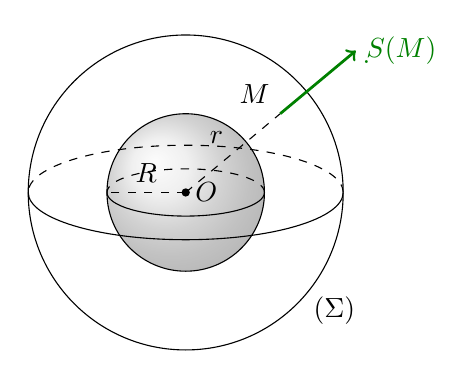
\begin{tikzpicture}[scale = 0.5]
 \shade[ball color = gray!40, opacity = 0.4] (0,0) circle (2cm); % couleur de la sphère et transparence
 \draw (0,0) circle (2cm); % contour de la sphère
  \draw (-2,0) arc (180:360:2 and 0.6); % section transversale de la sphère
  \draw[dashed] (2,0) arc (0:180:2 and 0.6); % section transversale de la sphère opposée
   \fill[fill=black] (0,0) circle (3pt) node[right]{$O$};% point central de la sphère
  \draw (0,0) circle (4cm); % contour de la sphère
  \draw (-4,0) arc (180:360:4 and 1.2); % section transversale de la sphère
  \draw[dashed] (4,0) arc (0:180:4 and 1.2); % section transversale de la sphère opposée
  \draw[dashed] (0,0)--(2 * 1.2, 2 * 1.0);
    \draw (1.2, 1.0) node[above left]{$r$};
    \draw[dashed] (0,0)--(-2, 0);
    \draw (-1, 0) node[above]{$R$};
  \draw[green!50!black,->, line width = 1] (2 * 1.2, 2 * 1.0)node[black, above left]{$M$} -- (2 * 1.8 * 1.2, 2 * 1.8 * 1.0) node[right]{$\d \Vec{\mc{S}}(M)$}; % vecteur rouge partant de (1.2,1.0)
  \draw (3,-3) node[right]{$(\Sigma)$};
       \end{tikzpicture}
\end{center}
\begin{solu}
On choisit d'utiliser les coordonnées sphériques.
\begin{enum}
\item \imp{Invariance} : La distribution de charges est invariante par rotation d'angle $\theta$ et $\varphi$. \eq{E(M) = E(r)}
\imp{Symétrie} : Tout plan passant par $O$ et $M$ est plan de symétrie de la distribution de charge donc $\E$ appartient à tous ces plans. \eq{\E(M) \propto \er}
\eq{\E(M) = E(r) \er}
\item \imp{Choix de la surface de Gauss} : $(\Sigma)$ est une sphère de rayon $r$ et de centre $O$. \eq{\oiint_{(\Sigma)} \E \ps \d \Vec{\mc{S}} = \oiint_{(\Sigma)} E(r) \oiint \d S = E(r) \ps 4 \pi r^2}
\item \imp{Théorème de Gauss} : \eq{\oiint_{(\Sigma)} \E \ps \d \Vec{\mc{S}} = \frac{Q_{\rm{int}}}{\varepsilon_{0}} }
Deux cas :
\begin{liste}
\item $r \geq R$ : \eq{Q_{\rm{int}} = \iiint_{S(O, R)} \rho \d \mc{V} = \rho \frac{4}{3}\pi R^3 = Q_{\rm{tot}}}
\eq{\E(M \notin S(O, R) ) = \frac{Q_{\rm{tot}}}{4 \pi  \varepsilon_{0} r^2 }\er }
\item $r<R$ : \eq{Q_{\rm{int}} = \iiint_{S(O, r)} \rho \d \mc{V} = \rho \frac{4}{3}\pi r^3}
Donc \eq{\E(M \in S(O, R) ) =  \frac{\rho r}{3 \varepsilon_{0}}\er = \frac{Q_{\rm{tot}}}{4 \pi  \varepsilon_{0} } \ps \frac{ r}{R^3}\er }
\end{liste}
\end{enum}

\begin{center}
\begin{tikzpicture}
\begin{axis}[
    axis lines = middle,
    x label style={at={(axis description cs:1.1,0)},anchor=east},
    y label style={at={(axis description cs:0,1.2)},anchor=north},
    xlabel = $r$,
    ylabel = $\E(r)$,
    ymin=0, ymax=5,
    xmin=0, xmax=10,
    xtick=\empty, ytick=\empty, % supprime les graduations
    color=black
]

\addplot [
    domain=0:3, 
    samples=100, 
    color=red,
    line width = 2
]
{x};
\addplot [
    domain=3:10, 
    samples=100, 
    color=red,
    line width = 2
]
{3*(3/x)^2};

\begin{scope}[on background layer]
    \fill[fill=red] (axis cs:3,3) circle (3pt);
    \draw[dashed, red, line width = 1] (axis cs:3,0)node[below]{$R$}--(axis cs:3,3)--(axis cs:0,3)node[left]{$\frac{Q_{\rm{tot}}}{4 \pi  \varepsilon_{0} R^2 }$};
\end{scope}
\end{axis}
\end{tikzpicture}
\end{center}

\end{solu}

\end{exemple}

\begin{prop}
Le champ $\E$ créé à l'extérieur d'une distribution de charge à symétrie sphérique est égal au champ crée par une charge ponctuelle située au centre de la sphère et concentrant toute la charge de la distribution.
\end{prop}

\begin{exemple}{Boule uniformément chargée en surface}
On considère une sphère de centre $O$ de rayon $R$ uniformément chargé en surface de densité surfacique de charge $\sigma > 0$.
Déterminer le champ électrostatique crée en tout point de l'espace.

\begin{solu}
L'étude des invariances et des symétries est identique \eq{\E(M) = E(r) \er.}
Le choix de la surface de Gauss $(\Sigma)$ est identique.
\eq{Q_{\rm{tot}} = 4 \pi R^2 \sigma}
\begin{liste}
\item $r \geq R$ : \eq{Q_{\rm{int}} = Q_{\rm{tot}}}
\eq{\E(M \notin S(O, R) ) = \frac{Q_{\rm{tot}}}{4 \pi  \varepsilon_{0} r^2 }\er }
\item $r<R$ : \eq{Q_{\rm{int}} = 0}
Donc \eq{\E(M \in S(O, R) ) =  \Vec{0} }
\end{liste}
\begin{remarque}
$\nv{E}$ est discontinue mais cela est possible car cette densité surfacique est une modélisation et n'a pas de réalité physique.
\end{remarque}
\end{solu}

\begin{center}
\begin{tikzpicture}
\begin{axis}[
    axis lines = middle,
    x label style={at={(axis description cs:1.1,0)},anchor=east},
    y label style={at={(axis description cs:0,1.2)},anchor=north},
    xlabel = $r$,
    ylabel = $\E(r)$,
    ymin=-0.2, ymax=5,
    xmin=-0.2, xmax=10,
    xtick=\empty, ytick=\empty, % supprime les graduations
    color=black
]

\addplot [
    domain=0:3, 
    samples=100, 
    color=red,
    line width = 2
]
{0};
\addplot [
    domain=3:10, 
    samples=100, 
    color=red,
    line width = 2
]
{3*(3/x)^2};

\begin{scope}[on background layer]
    \draw[dashed, red, line width = 1] (axis cs:3,0)node[below]{$R$}--(axis cs:3,3)--(axis cs:0,3)node[left]{$\frac{\sigma}{\varepsilon_{0}}$};
\end{scope}
\begin{scope}[overlay]
    \fill[white] (axis cs:3,0) circle (3pt);
    \draw[red, line width =1] (axis cs:3,0) circle (3pt);
    \fill[white] (axis cs:3,3) circle (3pt);
    \draw[red, line width =1] (axis cs:3,3) circle (3pt);
\end{scope}
\end{axis}
\end{tikzpicture}
\end{center}


\end{exemple}


\begin{exemple}{Cylindre infini uniformément chargé en volume}
On considère un cylindre infini d'axe $(Oz)$, de rayon $R$ uniformément chargé en volume de densité volumique de charge $\rho > 0$.
Déterminer le champ électrostatique crée en tout point de l'espace.

\begin{center}
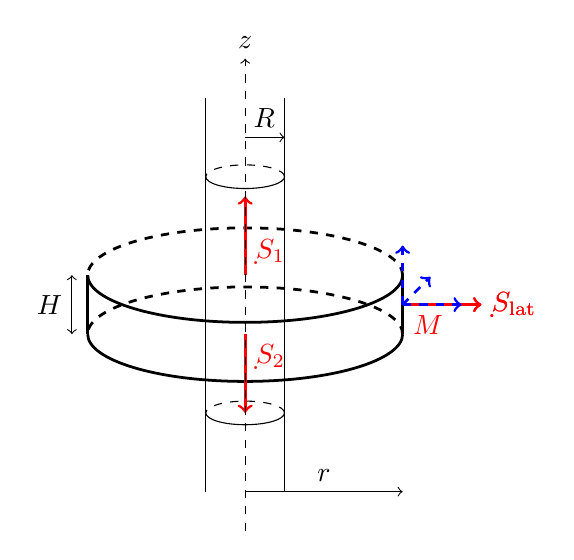
\begin{tikzpicture}[scale = 1]
\def\h{3} % hauteur du cylindre
  \def\r{0.5} % rayon de la base du cylindre
 \def\H{0.75} % hauteur du cylindre
  \def\R{2} % rayon de la base du cylindre
  
    \draw[dashed] (\r,0) arc (0:180:{\r} and {0.3 * \r}); % section transversale de la sphère opposée
    \draw (-\r,0) arc (180:360:{\r} and {0.3 * \r}); % section transversale de la sphère opposée
    \draw[dashed] (\r,\h) arc (0:180:{\r} and {0.3 * \r}); % section transversale de la sphère opposée
    \draw (-\r,\h) arc (180:360:{\r} and {0.3 * \r}); % section transversale de la sphère
    
     \draw[dashed, line width = 1] (\R,1) arc (0:180:{\R} and {0.3 * \R}); % section transversale de la sphère opposée
    \draw[line width = 1] (-\R,1) arc (180:360:{\R} and {0.3 * \R}); % section transversale de la sphère opposée
    \draw[dashed, line width = 1] (\R,{\H+1}) arc (0:180:{\R} and {0.3 * \R}); % section transversale de la sphère opposée
    \draw[line width = 1] (-\R,{\H+1}) arc (180:360:{\R} and {0.3 * \R}); % section transversale de la sphère 
    
    \draw (-\r,-1) -- (-\r,{\h+1}) ;
    \draw (\r,-1) -- (\r,{\h+1}) ;
    \draw[line width = 1] (-\R,1) -- (-\R,{\H+1}) ;
    \draw[line width = 1] (\R,1) -- (\R,{\H+1}) ;
    
    \draw[->] (0,3.5) -- (\r, 3.5) node[above left]{$R$};
    
    \draw[->] (0,-1) -- (\R, -1);
    \draw ({\R/2}, -1) node[above]{$r$};
    
    \draw[->, red, line width = 1] (\R, {2.75/2})node[below right]{$M$} -- ({\R+1}, {2.75/2})node[right]{$\d \Vec{\mc{S}}_{\rm{lat}}$};
    
    \draw[->, red, line width = 1] (\R, {2.75/2}) -- ({\R+1}, {2.75/2})node[right]{$\d \Vec{\mc{S}}_{\rm{lat}}$};
    \draw[->, red, line width = 1] (0, {\H + 1})node[above right]{$\d \Vec{\mc{S}}_{1}$}-- (0, {\H + 2});
    \draw[->, red, line width = 1] (0, {1})node[below right]{$\d \Vec{\mc{S}}_{2}$}-- (0, {0});
    
    \draw[->, dashed] (0,-1.5) -- (0, 4.5)node[above]{$z$};
    
     \draw[->, dashed, blue, line width = 1] (\R, {2.75/2}) -- ({\R+0.75}, {2.75/2})node[below]{$\er$};
     \draw[->, dashed, blue, line width = 1] (\R, {2.75/2}) -- ({\R}, {2.75/2 + 0.75})node[above]{$\ez$};
    \draw[->, dashed, blue, line width = 1] (\R, {2.75/2}) -- ({\R + 0.5*cos(45)}, {2.75/2 + 0.5*sin(45)})node[right]{$\et$};
    
    \draw[<->] ({-1.1 * \R}, 1)--({-1.1 * \R},{\H+1});
    \draw ({-1.1 * \R}, {\H/2+1}) node[left]{$H$};

\end{tikzpicture}
\end{center}
\begin{solu}
On choisit d'utiliser les coordonnées cylindrique.
\begin{enum}
\item \imp{Invariance} : La distribution de charges est invariante par rotation d'angle $\theta$ et par translation selon $z$. \eq{\E(M) = \E(r)}
\imp{Symétrie} : Les plans $(M, \er,\et)$ et $(M, \er,\ez)$ sont plans de symétrie de la distribution de charge, le champ électrostatique $\E$ appartient donc à ces deux plans $\E(M) \propto \er$.
\eq{\E(M) = E(r) \er}
\item \imp{Choix de la surface de Gauss} : On choisit une surface cylindrique de rayon $r$ d'axe $(Oz)$ que l'on ferme par deux surfaces parallèles $\mc{S}_{1}$ et $\mc{S}_{2}$ qui sont orthogonales à $(Oz)$ telles que $\E \perp \d \Vec{\mc{S}}$. Ces deux surface sont séparés d'une distance $H$. \eq{\phi_{1}= \phi_{2} = 0}
 \eq{\phi_{\rm{tot}} = \oiint_{(\Sigma) = (\mc{S}_{1}) \cup (\mc{S}_{2}) \cup (\mc{S}_{\rm{lat}})} \E \ps \d \Vec{\mc{S}} = \phi_{\rm{lat}}=  E(r) \oiint_{(\mc{S}_{\rm{lat}})} \d S = E(r) \ps 2 \pi r H}
\item \imp{Théorème de Gauss} : \eq{\oiint_{(\Sigma)} \E \ps \d \Vec{\mc{S}} = \frac{Q_{\rm{int}}}{\varepsilon_{0}} }
Deux cas :
\begin{liste}
\item $r \geq R$ : \eq{Q_{\rm{int}} = \rho \pi R^2 H}
\eq{\E(r \geq R ) = \frac{\rho}{2  \varepsilon_{0}} \frac{R^2}{r}\er }
\item $r<R$ : \eq{Q_{\rm{int}} = \rho \pi r^2 H}
Donc \eq{\E(r < R ) = \frac{\rho}{2  \varepsilon_{0}} r \er  }
\end{liste}
\end{enum}

\begin{center}
\begin{tikzpicture}
\begin{axis}[
    axis lines = middle,
    x label style={at={(axis description cs:1.1,0)},anchor=east},
    y label style={at={(axis description cs:0,1.2)},anchor=north},
    xlabel = $r$,
    ylabel = $\E(r)$,
    ymin=-0.2, ymax=5,
    xmin=-0.2, xmax=10,
    xtick=\empty, ytick=\empty, % supprime les graduations
    color=black
]

\addplot [
    domain=0:3, 
    samples=100, 
    color=red,
    line width = 2
]
{x};
\addplot [
    domain=3:10, 
    samples=100, 
    color=red,
    line width = 2
]
{3*(3/x)^2};

\begin{scope}[on background layer]
    \draw[dashed, red, line width = 1] (axis cs:3,0)node[below]{$R$}--(axis cs:3,3)--(axis cs:0,3)node[left]{$\frac{\rho_{0} R}{2 \varepsilon_{0}}$};
    \fill[fill=red] (axis cs:3,3) circle (3pt);
\end{scope}
\end{axis}
\end{tikzpicture}
\end{center}

\end{solu}

\end{exemple}

\begin{exemple}{Plan uniformément chargé en surface}
On considère un plan $(Oxy)$ uniformément chargé en surface $\sigma$ ($\sigma > 0$). Déterminer le champ électrostatique créé en tout point de l'espace.

\begin{center}
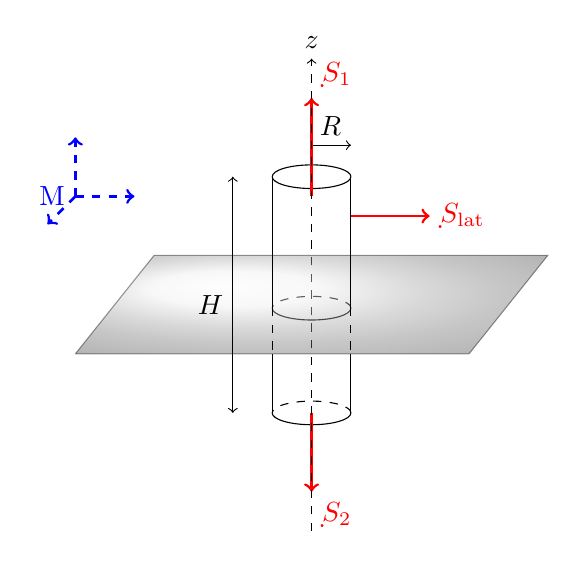
\begin{tikzpicture}[scale = 1]
\def\h{3} % hauteur du cylindre
  \def\r{0.5} % rayon de la base du cylindre
 \def\H{0.75} % hauteur du cylindre
  \def\R{-3} % rayon de la base du cylindre
  
    \draw[dashed] (\r,0) arc (0:180:{\r} and {0.3 * \r}); % section transversale de la sphère opposée
    \draw (-\r,0) arc (180:360:{\r} and {0.3 * \r}); % section transversale de la sphère opposée
    \draw (\r,\h) arc (0:180:{\r} and {0.3 * \r}); % section transversale de la sphère opposée
    \draw (-\r,\h) arc (180:360:{\r} and {0.3 * \r}); % section transversale de la sphère
    \draw[dashed] (\r,1.33) arc (0:180:{\r} and {0.3 * \r}); % section transversale de la sphère opposée
    \draw (-\r,1.33) arc (180:360:{\r} and {0.3 * \r}); % section transversale de la sphère
    
    
    \draw[->] (0,3.4) -- (\r, 3.4) node[above left]{$R$};
   
    

    
    \draw[->, red, line width = 1] (\r, {(\h+1+1)/2}) -- ({\r+1}, {(\h+1+1)/2})node[right]{$\d \Vec{\mc{S}}_{\rm{lat}}$};
    \draw[<-, red, line width = 1] (0, {\h + 1})node[above right]{$\d \Vec{\mc{S}}_{1}$}-- (0, {\H + 2});
    \draw[<-, red, line width = 1] (0, {-1})node[below right]{$\d \Vec{\mc{S}}_{2}$}-- (0, {0});
    
    \draw[->, dashed] (0,-1.5) -- (0, 4.5)node[above]{$z$};
    
    \draw[ball color = gray!20, opacity = 0.4] (-3,0.75) -- (2,0.75) -- (3,2) -- (-2,2)-- (-3,0.75);
    
     \draw[->, dashed, blue, line width = 1] (\R, {2.75})node[left]{M} -- ({\R+0.75}, {2.75})node[right]{$\ey$};
     \draw[->, dashed, blue, line width = 1] (\R, {2.75}) -- ({\R}, {2.75 + 0.75})node[right]{$\ez$};
    \draw[->, dashed, blue, line width = 1] (\R, {2.75}) -- ({\R - 0.5*cos(45)}, {2.75  -0.5*sin(45)})node[below left]{$\ex$};
    
    \draw[<->] ({-2 * \r}, 0)--({-2* \r},{\h});
    \draw ({-2 * \r}, {\H/2+1}) node[left]{$H$};
    
     \draw (-\r,0) -- (-\r,0.75) ;
    \draw (\r,0) -- (\r,0.75) ;
    
    \draw[dashed] (-\r, 1.33) -- (-\r,0.75);
    \draw[dashed] (\r, 1.33) -- (\r,0.75);
    
    \draw (-\r,1.33) -- (-\r,{\h}) ;
    \draw (\r,1.33) -- (\r,{\h}) ;

\end{tikzpicture}
\end{center}

\begin{solu}
\begin{enum}
\item \imp{Invariance} : La distribution de charge est \imp{invariante} par translation selon $(Ox)$ et $(Oy)$ \eq{\E(M) = \E(z).}
\noindent \imp{Symétrie} : Les plans $(M, \ex, \ez)$ et $(M,\ey,\ez)$ sont plans de symétrie de la distribution de charge donc $\E$ appartient à ces plans $\E \propto \ez$ \eq{\E(M) = E(z) \ez.}
\noindent $(O, \ex, \ey)$ est plan de symétrie de la distribution de charge donc du champ $\E$ \eq{\E(-z) = - \E(z)}
\item \imp{Choix de la surface de Gauss} : On choisit une portion d'équipotentielle $\mc{S}_{1}$ e, ($z=\cst$) et $\mc{S}_{2}$ son symétrique par rapport à $(O, \ex, \ey)$ en ($z = -\cst$) et on ferme par une surface $\mc{S}_{\rm{lat}}$ orthogonale à $\E$. \begin{align*}
\phi_{\rm{tot}} &= \oiint_{(\Sigma) = (\mc{S}_{1}) \cup (\mc{S}_{2}) \cup (\mc{S}_{\rm{lat}})} \E \ps \d \Vec{\mc{S}} = \phi_{1} + \phi_{2} + \canc{\phi_{\rm{lat}}}\\
&=  E(z) \iint_{(\mc{S}_{1})} \d S_{1} - E(-z) \iint_{(\mc{S}_{2})} \d S_{2} \\
&= E(z) \iint_{(\mc{S}_{1})} \d S_{1} + E(z) \iint_{(\mc{S}_{2})} \d S_{2}\\
&= 2 E(z) \pi R^2
\end{align*}
\item \imp{Théorème de Gauss} : \eq{\oiint_{(\Sigma) = (\mc{S}_{1}) \cup (\mc{S}_{2}) \cup (\mc{S}_{\rm{lat}})} \E \ps \d \Vec{\mc{S}} = \frac{Q_{\rm{int}}}{\varepsilon_{0}} = \pi R^2 \frac{\sigma}{\varepsilon_{0}} }
\eq{\E(M) = \frac{\sigma}{2\varepsilon_{0}} \quad \quad \quad \textnormal{Si $z > 0$}}
\eq{\E(M) = -\frac{\sigma}{2\varepsilon_{0}} \quad \quad \quad \textnormal{Si $z  < 0$}}
\end{enum}

\begin{remarque}
$\E$ est discontinue à la traversée de la surface chargée. La discontinuité vaut $\frac{\sigma}{\varepsilon_{0}}$. Ce résultat est en fait généralisable et nous verrons son origine plus tard.
\end{remarque}

\begin{center}
\begin{tikzpicture}
\begin{axis}[
    axis lines = middle,
    x label style={at={(axis description cs:1.1,0.5)},anchor=east},
    y label style={at={(axis description cs:0.5,1.1)},anchor=north},
    xlabel = $z$,
    ylabel = $E(z)$,
    ymin=-2, ymax=2,
    xmin=-4, xmax=4,
    xtick=\empty, ytick=\empty, % supprime les graduations
    color=black
]
\addplot [
    domain=-4:0, 
    samples=100, 
    color=red,
    line width = 2
]
{-1};

\addplot [
    domain=0:4, 
    samples=100, 
    color=red,
    line width = 2
]
{1};


\begin{scope}[on background layer]
     \draw[red] (axis cs:0,1) node[left]{$\frac{\sigma}{2 \varepsilon_{0}}$};
    \draw[red] (axis cs:0,-1) node[right]{$-\frac{\sigma}{2 \varepsilon_{0}}$};
\end{scope}
\begin{scope}[overlay]
    \fill[white] (axis cs:0,1) circle (3pt);
    \draw[red, line width =1] (axis cs:0,1) circle (3pt);
    \fill[white] (axis cs:0,-1) circle (3pt);
    \draw[red, line width =1] (axis cs:0,-1) circle (3pt);
\end{scope}
\end{axis}
\end{tikzpicture}
\end{center}


\end{solu}

\end{exemple}

\begin{theorem}[Relation de passage électrostatique]
A la traversée d'une surface chargé $\mc{S}$ de densité surfacique de charge $\sigma$, la composante normale du champ $\E$ subit une discontinuité et la composante tangentielle est continue telle que : \eq{\E_{2}(M) - \E_{1}(M) = \frac{\sigma(M)}{\varepsilon_{0}} \Vec{n}_{1 \Ar 2}.}
\begin{center}
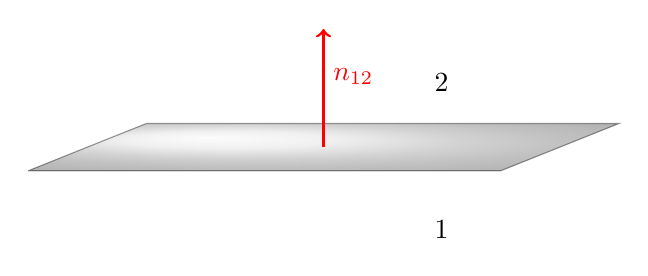
\begin{tikzpicture}[scale=1.5]
  \draw[ball color = gray!40, opacity = 0.4] (0,0) -- (4,0) -- (5,0.4) -- (1,0.4)-- (0,0);
  \draw (3.5,-0.5) node{$1$};
  \draw (3.5, 0.75) node{$2$};
    \draw[->, red, line width = 1] (2.5, 0.2)-- (2.5, 1.2);
    \draw[red] (2.5, 0.8) node[right]{$\Vec{n}_{1 \Ar 2}$};
\end{tikzpicture}
\end{center}
$\Vec{n}_{1 \Ar 2}$ est le vecteur unitaire, orthogonal à la surface, allant de $1$ vers $2$.
\end{theorem}

\subsection{Condensateur plan} 

\parag{Capacité}
\noindent Un condensateur est constitué de deux armatures parallèles de surface $\mc{S}$ distante de $e$ ( $e \ll \sqrt{\mc{S}}$ ) de sorte que l'on peut peut négliger les effets de bord.
Une armature porte la charge $+Q$ et l'autre la charge $-Q$.

\begin{center}
\begin{tikzpicture}[scale = 2]
\foreach \j in {-1.8, -1.6,...,1.8}
 	\draw[postaction={decorate,decoration={markings, mark=at position 0.5 with {\arrow{>}}}}, blue!50!black, line width=1] ({\j},-0.2) to[out=90,in=-90] ({\j}, 0.2);
	\draw[postaction={decorate,decoration={markings, mark=at position 0.5 with {\arrow{>}}}}, blue!50!black, line width=1] (-2,-0.2) to[out=120,in=-120] (-2, 0.2);
	\draw[postaction={decorate,decoration={markings, mark=at position 0.5 with {\arrow{>}}}}, blue!50!black, line width=1] (2,-0.2) to[out=70,in=-70] (2, 0.2);


\draw[color=green!60!black,line width = 3] (-2,0.2) -- (2,0.2)node[midway, above right]{$-Q$}node[midway, above left]{$V_{1}$};
\draw[color=green!60!black,line width = 3] (0,0.5) -- (0,0.2);
\draw[color=red!80!black,line width = 3] (-2,-0.2) -- (2,-0.2)node[midway, below right]{$+Q$}node[midway, below left]{$V_{2}$};
\draw[color=red!80!black,line width = 3] (0,-0.5) -- (0,-0.2);

\draw[->, line width = 1] (-2.5,0.5) -- (-2.5,-0.5)node[midway, left]{$U$};
\draw[<->, line width = 1] (2.5,0.2) -- (2.5,-0.2)node[midway, right]{$e$};
\end{tikzpicture}
\end{center}

\noindent Une armature est au potentiel $V_{1}$ et l'autre $V_{2}$ de sorte que la tension ou différence de potentiel $U$ aux borne du condensateur soit \eq{U = V_{2} - V_{1}}

\begin{definition}
La capacité du condensateur ainsi formée est \eq{C = \frac{Q}{U}}
et est exprimée en $\SI{}{F}$ (Farad).
$Q$ étant la charge à l'armature chargé positivement et $U$ étant aussi compté positivement.
\end{definition}

\begin{remarque}
$Q$ étant proportionnel à $U$, la capacité $C$ ne dépend pas de $U$ et de $Q$ mais uniquement de la géométrie du condensateur, y compris ceux à géométrie cylindrique et sphérique.
\end{remarque}

\begin{exemple}{Capacité d'un condensateur plan}

Déterminer la capacité $C$ d'un condensateur plan chargé en surface de densité surfacique de charge $\sigma$ ($\sigma > 0$) en considérant les armatures comme des plans infinis séparé de la distance $e$.
\begin{center}
\begin{tikzpicture}[scale = 1.5]
\foreach \j in {-3.8, -3.6,...,3.8}
 	\draw[postaction={decorate,decoration={markings, mark=at position 0.5 with {\arrow{>}}}}, blue!50!black, line width=1] ({\j},-0.2) to[out=90,in=-90] ({\j}, 0.2);



\draw[color=green!60!black,line width = 3] (-4,0.2) -- (4,0.2)node[midway, above right]{$-Q = -\sigma S$}node[midway, above left]{$V_{1}$};
\draw[color=green!60!black,line width = 3] (0,0.5) -- (0,0.2);
\draw[color=red!80!black,line width = 3] (-4,-0.2) -- (4,-0.2)node[midway, below right]{$+Q = \sigma S$}node[midway, below left]{$V_{2}$};
\draw[color=red!80!black,line width = 3] (0,-0.5) -- (0,-0.2);


\draw[->, line width = 1] (2.5,-1) -- (2.5,1)node[above]{$z$};
\draw(2.5,-0.2)node{$+$}node[below right]{$O$};
\draw(2.5,0.2)node{$+$}node[above right]{$e$};
\end{tikzpicture}
\end{center}

\begin{solu}
\noindent Appliquons le principe de superposition \eq{\E = \E_{1} + \E_{2}.}
\noindent Où $\E_{1}$ est le champ créé par l'armature $1$ 
\eq{\E_{1} = -\frac{\sigma}{2\varepsilon_{0}}\ez \quad \quad \quad \textnormal{(z>e)}}
\eq{\E_{1} =  \frac{\sigma}{2\varepsilon_{0}}\ez \quad \quad \quad \textnormal{(z<e).}}
$\E_{2}$ est le champ créé par l'armature $2$ 
\eq{\E_{2} = \frac{\sigma}{2\varepsilon_{0}}\ez\quad \quad \quad \textnormal{(z>0)}}
\eq{\E_{2} = - \frac{\sigma}{2\varepsilon_{0}}\ez \quad \quad \quad \textnormal{(z<0).}}

\noindent Ainsi le champ total $\E$ est pour $z\in \[0;e \]$ \eq{\E(z\in \[0;e \]) = \frac{\sigma}{\varepsilon_{0}}\ez}
pour $z \notin  \[0;e \]$ \eq{\E(z\notin \[0;e \]) = \vv{0}.}

\noindent La tension $U$ entre les deux armatures est donc
\begin{align*}
U &= V_{2} - V_{1} = \int^2_{1} \d V = - \int^1_{2}\d V\\
&= \int^1_{2} \E \ps \dl = \frac{\sigma}{\varepsilon_{0}} \int^{e}_{0} \d \ell = \frac{\sigma e}{\varepsilon_{0}} = \frac{Q e}{\mc{S} \varepsilon_{0}}
\end{align*}
On en déduit \eq{C = \frac{\varepsilon_{0} mc{S}}{e}}
\end{solu}

\end{exemple}

\begin{theorem}
La capacité $C$ d'un condensateur plan de surface $\mc{S}$ et d'épaisseur $e$ est \eq{C = \frac{\varepsilon_{0} mc{S}}{e}.}

\end{theorem}

\begin{odg}
$\varepsilon_{0} = \SI{8.85e-12}{F.m^{-1}} \simeq \SI{e-11}{F.m^{-1}}$ \\
$S \simeq \SI{1}{cm^2} \simeq \SI{e-4}{m^2}$\\
$e \simeq \SI{0.1}{mm} \simeq \SI{e-4}{m}$\\
$C \simeq \SI{e-11}{F}$

\end{odg}

\begin{remarque}
Pour avoir un condensateur de plus grande capacité, on met un diélectrique entre les armatures de permittivité relative $\varepsilon_{r}$ ($\varepsilon_{r} \Lar 1000$)
\eq{C = \frac{\varepsilon_{0}\varepsilon_{r} mc{S}}{e}.}
\end{remarque}

\parag{Aspect énergétique} : La charge stockée dans un condensateur lors de sa charge de durée $t_{c}$ est 
\begin{align*}
\mc{E} &= \int^{t_{c}}_{0} \mc{P}(t) \d t =  \int^{t_{c}}_{0} u(t) i(t) \d t \\
&=  \int^{t_{c}}_{0} C u(t) \dd{u}{t}(t) \d t \\
&= \int^{U}_{0} C u \d u\\
&= \frac{1}{2} C U^2
\end{align*}

\noindent Pour un condensateur plan $C = \frac{\varepsilon_{0} mc{S}}{e}$ et $\abs{U} = e E$ donc 
\begin{align*}
\mc{E} = \frac{1}{2} \frac{\varepsilon_{0} \mc{S}}{e} e^2 E^2 = \frac{1}{2} \varepsilon_{0} E^2 (\mc{S}e).
\end{align*}
Le volume $\mc{V} = \mc{S}e$ entre les armatures apparaît.

\begin{theorem}{Généralisation}
La densité volumique d'énergie électrique, exprimée en $\SI{}{J.m^-3}$ est \eq{u_{\rm{elec}}(M) = \frac{1}{2} \varepsilon_{0} \rVert \E(M) \lVert^2}
telle que l'énergie électrique $\d \mc{E}_{\rm{elec}}(M)$ contenue dans un petit volume $\d \mc{V}(M)$ en $M$ est \eq{\d \mc{E}_{\rm{elec}}(M) =u_{\rm{elec}}(M) \d \mc{V}}
\end{theorem}

\subsection{Analogie avec le champ gravitationnel} 

\begin{center}
\renewcommand{\arraystretch}{2.5}
\begin{tabular}{|c|c|c|}
\hline
 & Electrostatique & Gravitation \\
\hline
Sources & Charges fixes & Masses \\
 & 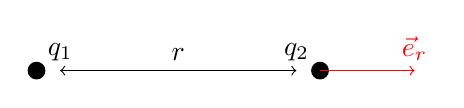
\begin{tikzpicture}[scale=1.5]
    \coordinate[label=above:$q_1$] (A) at (0,0);
    \coordinate[label=above:$q_2$] (B) at (2,0);
    \coordinate[label={[above,text=red]:$\vec{e}_r$}] (C) at (3,0);
    \draw[<->] (A) -- node[midway,above] {$r$} (B);
    \filldraw[black] (A) ++(-0.2,0) circle (2pt);
    \filldraw[black] (B) ++(0.2,0) circle (2pt);
    \draw[->,red] (B) ++(0.2,0) -- (C);
  \end{tikzpicture}
 & 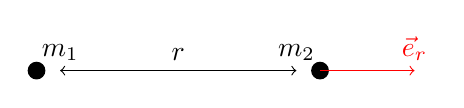
\begin{tikzpicture}[scale=1.5]
    \coordinate[label=above:$m_1$] (A) at (0,0);
    \coordinate[label=above:$m_2$] (B) at (2,0);
    \coordinate[label={[above,text=red]:$\vec{e}_r$}] (C) at (3,0);
    \draw[<->] (A) -- node[midway,above] {$r$} (B);
    \filldraw[black] (A) ++(-0.2,0) circle (2pt);
    \filldraw[black] (B) ++(0.2,0) circle (2pt);
    \draw[->,red] (B) ++(0.2,0) -- (C);
  \end{tikzpicture} \\
\hline
Force & $\displaystyle \vec{F}_{q_1\to q_2}=\frac{q_1\cdot q_2}{4\pi\varepsilon_0 r^2}\vec{e}_r$ & $ \displaystyle \vec{F}_{m_1\to m_2}=-\mc{G}\frac{m_1\cdot m_2}{r^2}\vec{e}_r$ \\
\hline
Champ créé par les sources & $\displaystyle \vec{E}_1(2)=\frac{\vec{F}_{q_1\to q_2}}{q_2}=\frac{q_1}{4\pi\varepsilon_0 r^2}\vec{e}_r$ & $\displaystyle \vec{G}_1(2)=\frac{\vec{F}_{m_1\to m_2}}{m_2}=-\mc{G}\frac{m_1}{r^2}\vec{e}_r$ \\
\hline
Théorème de Gauss & $\displaystyle \oiint_{(\Sigma)}\vec{E}\cdot\mathrm{d}\Vec{\mc{S}}=\frac{Q_\mathrm{int}}{\varepsilon_0}$ & $\displaystyle \oiint_{(\Sigma)}\vec{G}\cdot\mathrm{d}\Vec{\mc{S}}=-4\pi\mc{G}M_\mathrm{int}$ \\
\hline
\end{tabular}
\end{center}


\begin{theorem}[Théorème de Gauss gravitationnel]

Le flux du champ gravitationnel à travers une surface fermée est égal à la somme des masses intérieure à cette surface multipliée par $-4 \pi \mc{G}$.
\eq{\oiint_{(\Sigma)} \Vec{G} \ps \d \Vec{\mc{S}} = -4 \pi \mc{G} M_{\rm{int}} }
On rappelle que la convention est d'orienté le vecteur surface infinitésimal $\d \Vec{\mc{S}}$ vers l'extérieur de la surface.
\end{theorem}

\begin{exemple}{Champ de gravitation}
On considère une boule de centre $O$, de rayon $R$, de masse volumique uniforme $\rho$ et de masse totale $M_{\rm{tot}}$. Déterminer le champ gravitationnel crée par cette distribution de masse en tout point de l'espace.
\begin{center}
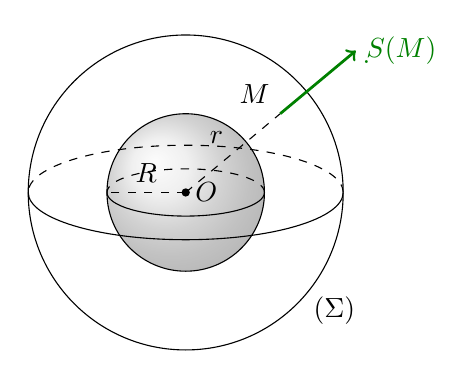
\begin{tikzpicture}[scale = 0.5]
 \shade[ball color = gray!40, opacity = 0.4] (0,0) circle (2cm); % couleur de la sphère et transparence
 \draw (0,0) circle (2cm); % contour de la sphère
  \draw (-2,0) arc (180:360:2 and 0.6); % section transversale de la sphère
  \draw[dashed] (2,0) arc (0:180:2 and 0.6); % section transversale de la sphère opposée
   \fill[fill=black] (0,0) circle (3pt) node[right]{$O$};% point central de la sphère
  \draw (0,0) circle (4cm); % contour de la sphère
  \draw (-4,0) arc (180:360:4 and 1.2); % section transversale de la sphère
  \draw[dashed] (4,0) arc (0:180:4 and 1.2); % section transversale de la sphère opposée
  \draw[dashed] (0,0)--(2 * 1.2, 2 * 1.0);
    \draw (1.2, 1.0) node[above left]{$r$};
    \draw[dashed] (0,0)--(-2, 0);
    \draw (-1, 0) node[above]{$R$};
  \draw[green!50!black,->, line width = 1] (2 * 1.2, 2 * 1.0)node[black, above left]{$M$} -- (2 * 1.8 * 1.2, 2 * 1.8 * 1.0) node[right]{$\d \Vec{\mc{S}}(M)$}; % vecteur rouge partant de (1.2,1.0)
  \draw (3,-3) node[right]{$(\Sigma)$};
       \end{tikzpicture}
\end{center}
\begin{solu}
On choisit d'utiliser les coordonnées sphériques.
\begin{enum}
\item \imp{Invariance} : La distribution de masse est invariante par rotation d'angle $\theta$ et $\varphi$. \eq{\vv{G}(M) = \vv{G}(r)}
\imp{Symétrie} : Tout plan passant par $O$ et $M$ est plan de symétrie de la distribution de masse donc $\vv{G}$ appartient à tous ces plans. \eq{\vv{G}(M) \propto \er}
\eq{\vv{G}(M) = G(r) \er}
\item \imp{Choix de la surface de Gauss} : $(\Sigma)$ est une sphère de rayon $r$ et de centre $O$. \eq{\oiint_{(\Sigma)} \\vv{G} \ps \d \Vec{\mc{S}} = \oiint_{(\Sigma)} G(r) \oiint \d S = G(r) \ps 4 \pi r^2}
\item \imp{Théorème de Gauss} : \eq{\oiint_{(\Sigma)} \vv{G} \ps \d \Vec{\mc{S}} = - 4 \pi \mc{G}M_{\rm{int}}}
Deux cas :
\begin{liste}
\item $r \geq R$ : \eq{M_{\rm{int}} = \iiint_{S(O, R)} \rho \d \mc{V} = \rho \frac{4}{3}\pi R^3 = M_{\rm{tot}}}
\eq{\vv{G}(M \notin S(O, R) ) = - \mc{G}\frac{M_{\rm{tot}}}{r^2 }\er }
\item $r<R$ : \eq{M_{\rm{int}} = \iiint_{S(O, r)} \rho \d \mc{V} = \rho \frac{4}{3}\pi r^3}
Donc \eq{\vv{G}(M \in S(O, R) ) =  -\mc{G}\frac{4}{3}\pi \rho r\er = -\mc{G} \frac{M_{\rm{tot}}}{ R^3 }  r \er }
\end{liste}
\end{enum}
\end{solu}

\end{exemple}

\section{Dipôle électrostatique}

\subsection{Définitions et approximations}

\parag{Distribution dipolaire}

\begin{definition}
Un \imp{dipôle électrostatique} est un ensemble de deux charges ponctuelles égales en valeur et opposées séparées par une distance $d$.
\begin{center}
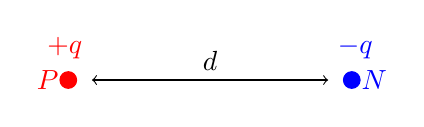
\begin{tikzpicture}[scale=1.5]
    \coordinate (A) at (0,0);
    \draw (A)++(0,0.1) node[above left,red]{$+q$};
    \draw (A)++(-0.2,0) node[left,red]{$P$};
        \coordinate(B) at (2,0);
     \draw (B)++(0,0.1) node[above right,blue]{$-q$};
     \draw (B)++(0.2,0) node[right,blue]{$N$};
    \draw[<->] (A) -- node[midway,above] {$d$} (B);
    \filldraw[red] (A) ++(-0.2,0) circle (2pt);
    \filldraw[blue] (B) ++(0.2,0) circle (2pt);
  \end{tikzpicture}
  \end{center}
\end{definition}

\begin{remarque}
On peut se ramener à ce cas lorsqu'il y a plus de deux charges et que $\sum_{i} q_{i} = 0$ en prenant $P$ le barycentre des charges positives et $N$ le barycentre des charges négatives.
\end{remarque}

\parag{Moment dipolaire}

\begin{definition}
Un dipôle électrostatique est caractérisé par son \imp{moment dipolaire} \eq{\Vec{p} = q \Vec{NP}}
exprimé en $\SI{}{C.m}$ et toujours orienté vers la charge positive.
\begin{center}
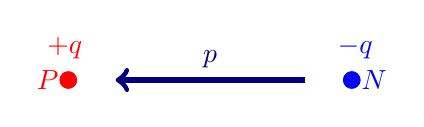
\begin{tikzpicture}[scale=1.5]
    \coordinate (A) at (0,0);
    \draw (A)++(0,0.1) node[above left,red]{$+q$};
    \draw (A)++(-0.2,0) node[left,red]{$P$};
        \coordinate(B) at (2,0);
     \draw (B)++(0,0.1) node[above right,blue]{$-q$};
     \draw (B)++(0.2,0) node[right,blue]{$N$};
    \draw[<-,blue!50!black,line width = 2] (0.2,0) -- node[midway,above] {$\vv{p}$} (1.8,0);
    \filldraw[red] (A) ++(-0.2,0) circle (2pt);
    \filldraw[blue] (B) ++(0.2,0) circle (2pt);
  \end{tikzpicture}
  \end{center}
\end{definition}


\begin{definition}
 Une \imp{molécule} est assemblage \imp{électriquement neutre} d'au moins deux atomes. Lorsque le moment dipolaire d'une molécule est non nulle, la molécule est qualifié de \imp{polaire} et s'il est nulle d'\imp{apolaire}.
 \end{definition}

\noindent Par exemple, la molécule de dihydrogène \ce{H2} est \imp{apolaire}.
\begin{center}
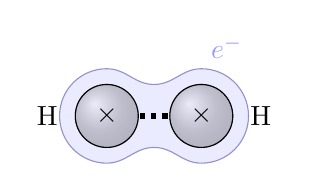
\begin{tikzpicture}[scale=2]
% Nuage électronique
\draw[blue!50!black,fill=blue!20!white,opacity=0.4] (0.6,0) 
    to[out=-90,in=0] (0.3,-0.3) 
    to[out=180,in=0] (0,-0.2) 
    to[out=180,in=0] (-0.3,-0.3) 
    to[out=180,in=-90] (-0.6,0);
    \draw[blue!50!black,fill=blue!20!white,opacity=0.4] (0.6,0) 
    to[out=90,in=0] (0.3,0.3) node[above right,blue!100!white]{$e^-$}
    to[out=180,in=0] (0,0.2) 
    to[out=-180,in=0] (-0.3,0.3) 
    to[out=180,in=90] (-0.6,0);

%Les liaisons
\draw[dotted, line width = 2] (-0.09,0) -- (0.1,0);

%Les atomes
\draw[ball color=gray, opacity=0.3] (0.3,0) circle (0.2cm) ;
\draw (0.3,0) circle (0.2cm);
\draw (0.3,0) node[right=0.5cm]{$\rm{H}$};
\draw (0.3,0) node{$\times$};
\draw[ball color=gray, opacity=0.3] (-0.3,0) circle (0.2cm) ;
\draw (-0.3,0) circle (0.2cm);
\draw (-0.3,0) node[left=0.5cm]{$\rm{H}$};
\draw (-0.3,0) node{$\times$};

\end{tikzpicture}
\end{center}

\noindent Alors que les molécules d'acide chlorhydrique \ce{HCl} et d'eau \ce{H2O} son \imp{polaires}.

\begin{center}
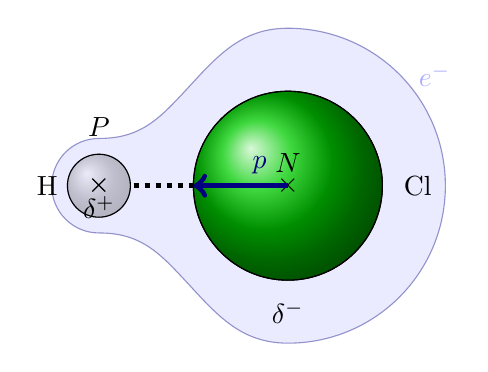
\begin{tikzpicture}[scale=2]
% Nuage électronique
\draw[blue!50!black,fill=blue!20!white,opacity=0.4] (1,0) 
    to[out=-90,in=0] (0,-1) 
    to[out=180,in=-45] (-0.75,-0.5) 
    to[out=135,in=0] (-1.2,-0.3) 
    to[out=180,in=-90] (-1.5,0);
    \draw[blue!50!black,fill=blue!20!white,opacity=0.4] (1,0) 
    to[out=90,in=0] (0,1) 
    to[out=180,in=45] (-0.75,0.5) 
    to[out=-135,in=0] (-1.2,0.3) 
    to[out=180,in=90] (-1.5,0);
    \draw (0.7,0.7) node[right=4pt,blue!80!white, ,opacity=0.4]{$e^-$} ;

%Les liaisons
\draw[dotted, line width = 2] (-0.98,0) -- (0,0);

%Les atomes
\draw[ball color=green!80!black] (0,0) circle (0.6cm) node[below=1.35cm] {$\delta^-$};
\draw (0,0) circle (0.6cm);
\draw (0,0) node[right=1.35cm]{$\rm{Cl}$};
\draw[ball color=gray, opacity=0.3] (-1.2,0) circle (0.2cm) ;
\draw (-1.2,0) circle (0.2cm);
\draw (-1.2,0) node[below=0.5, black] {$\delta^+$};
\draw (-1.2,0) node[left=0.4cm]{$\rm{H}$};
\draw (0,0) node{$\times$} node[above=1.35]{$N$};
\draw (-1.2,0) node{$\times$};
\draw (-1.2,0)node{$\times$}  node[above=0.5cm]{$P$};

%Le dipôle
\draw[->,blue!50!black,line width = 2] (0,0) -- node[pos=0.3, above]{$\vv{p}$} (-0.6,0);
\end{tikzpicture}
\end{center}




\begin{center}
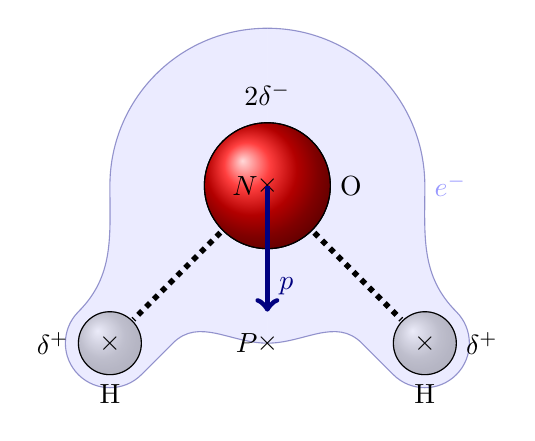
\begin{tikzpicture}[scale=2]

% Nuage électronique
\draw[blue!50!black,fill=blue!20!white,opacity=0.4] (0,1) 
    to[out=0,in=90] (1,0) node[right,blue!100!white]{$e^-$} 
    to[out=-90,in=135] (1.2,-0.8) 
    to[out=-45,in=45] (1.2,-1.2) 
    to[out=-135,in=-45] (0.8,-1.2)
    to[out=135,in=135] (0.6,-1)
    to[out=135,in=0] (0,-1);
\draw[blue!50!black,fill=blue!20!white,opacity=0.4] (0,1) 
    to[out=180,in=90] (-1,0) 
    to[out=-90,in=45] (-1.2,-0.8) 
    to[out=-135,in=135] (-1.2,-1.2) 
    to[out=-45,in=-135] (-0.8,-1.2)
    to[out=45,in=-135] (-0.6,-1)
    to[out=45,in=-180] (0,-1);
%Les liaisons
\draw[dotted, line width = 2] (0,0) -- (-0.85,-0.85);
\draw[dotted, line width = 2] (0,0) -- (0.85,-0.85);

%Les atomes
\draw[ball color=red] (0,0) circle (0.4cm) node[above=0.9cm] {$2\delta^-$};
\draw (0,0) circle (0.4cm);
\draw (0,0) node[right=0.8cm]{$\rm{O}$};
\draw[ball color=gray, opacity=0.3] (-1,-1) circle (0.2cm) ;
\draw (-1,-1) circle (0.2cm);
\draw (-1,-1) node[left=0.4cm, black] {$\delta^+$};
\draw[ball color=gray, opacity=0.3] (1,-1) circle (0.2cm);
\draw (1,-1) circle (0.2cm);
\draw (1,-1) node[below=0.4cm]{$\rm{H}$};
\draw (1,-1) node[right=0.4cm, black] {$\delta^+$};
\draw (-1,-1) node[below=0.4cm]{$\rm{H}$};
\draw (0,0) node{$\times$} node[left]{$N$};
\draw (1,-1) node{$\times$};
\draw (-1,-1) node{$\times$};
\draw (0,-1)node{$\times$}  node[left]{$P$};

%Le dipôle
\draw[->,blue!50!black,line width = 2] (0,0) -- node[pos=0.8, right]{$\vv{p}$} (0,-0.8);
\end{tikzpicture}
\end{center}

\begin{odg}
$\nv{p} = q d$

\noindent Pour une molécule, $q \simeq \SI{e-19}{C}$ et $d\simeq \SI{e-10}{m}$ d'où $\nv{p} \simeq \SI{e-29}{C.m}$

\noindent C'est pourquoi les chimistes utilisent le \it{Debye}, $\SI{1}{D} = \frac{1}{3} \cdot \SI{e-29}{C.m}$

\begin{liste}
\item $\nv{p}(\ce{H20}) = \SI{1.85}{D}$ 
\item $\nv{p}(\ce{HCl}) = \SI{1.08}{D}$ 
\end{liste}

\end{odg}

\parag{Approximation dipolaire}

\begin{definition}
L'\imp{approximation dipolaire} consiste à étudier le champ/potentiel créé par le dipôle à une distance $r$ très grande devant la taille caractéristique $d$ du dipôle \eq{r \gg d.}

\begin{center}
\begin{tikzpicture}[scale=0.4]
    \coordinate (A) at (0,0);
    \coordinate (C) at (11,10);
    \draw (A)++(0,0.1) node[above left,red]{$+q$};
    \draw (A)++(-0.2,0) node[left,red]{$P$};
        \coordinate(B) at (2,0);
     \draw (B)++(0,0.1) node[above right,blue]{$-q$};
     \draw (B)++(0.2,0) node[right,blue]{$N$};
    \draw[<->] (A) -- node[midway,below] {$d$} (B);
    \filldraw[red] (A) ++(-0.2,0) circle (2pt);
    \filldraw[blue] (B) ++(0.2,0) circle (2pt);
    \draw[dashed,line width = 2, green!50!black] (1,0)--node[green!50!black,midway,above left] {$r$} (C);
    \draw (C) node[above left]{$M$};
    \draw[->, red, line width = 1] (C) -- ++(1,1)node[right]{$\er$}; 
    \draw[->, red, line width = 1] (C) -- ++(1,-1)node[right]{$\et$}; 
     \draw[<-,blue!50!black,line width = 2] (0.2,-2) -- node[midway,below=2pt] {$\vv{p}$} (1.8,-2);
  \end{tikzpicture}
  \end{center}


\end{definition}

\begin{remarque}
On pourra alors faire des \acl{DLs} en $\frac{d}{r}$.
\end{remarque}



\subsection{Potentiel et champ crée par un dipôle électrostatique}

\parag{Potentiel créé par le dipôle}

\begin{center}
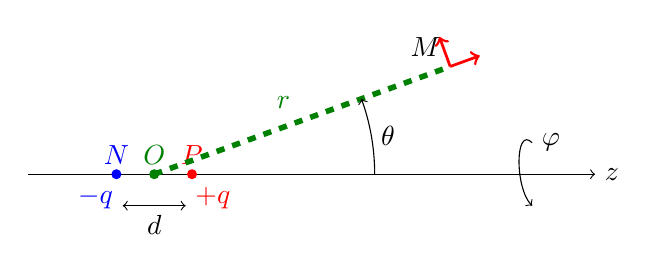
\begin{tikzpicture}[scale=0.4]
\draw[->] (-3,0)--(15,0)node[right]{$z$};
    \coordinate (A) at (0,0);
    \coordinate (C) at ({1+ 10 * cos(20)}, {10 * sin(20)});
    \draw (A)++(0,-0.1) node[below left,blue]{$-q$};
    \draw (A)++(-0.2,0) node[above,blue]{$N$};
        \coordinate(B) at (2,0);
     \draw (B)++(0,-0.1) node[below right,red]{$+q$};
     \draw (B)++(0.2,0) node[above,red]{$P$};
    \draw[<->] (0,-1) -- node[midway,below] {$d$} (2,-1);
    \filldraw[blue] (A) ++(-0.2,0) circle (4pt);
    \filldraw[green!50!black] (1,0)node[above]{$O$} circle (4pt);
    \filldraw[red] (B) ++(0.2,0) circle (4pt);
    \draw[dashed,line width = 2,green!50!black] (1,0)--node[green!50!black,midway,above left] {$r$} ({1+ 10 * cos(20)}, {10 * sin(20)});
    \draw (C) node[above left]{$M$};
    \draw[->, red, line width = 1] (C) -- ++({cos(20)}, {sin(20)})node[right]{$\er$}; 
    \draw[->, red, line width = 1] (C) -- ++({cos(110)}, {sin(110)})node[right]{$\et$}; 
    \draw[->] (8,0) arc[start angle=0, end angle=20, radius=7]node[midway,right]{$\theta$}; % arc de cercle et symbole theta;
    \draw[->, in=135, out=135] (13,1)node[right]{$\varphi$} to (13,-1);

     \end{tikzpicture}
  \end{center}
  
  Pla\c cons nous en coordonnées sphérique $(O,\er,\et,\ep)$ telles que \eq{r = \vv{OM} \quad \quad \quad \quad  \quad \theta = (\ez,\er).}
  
  \noindent Calculons le potentiel au point $M$ :
  \begin{align*}
  V(M) &= \frac{q}{4\pi \varepsilon_{0} \nv{PM}} - \frac{q}{4\pi \varepsilon_{0} \nv{NM}}\\
  & = \frac{q}{4\pi \varepsilon_{0}} \( \frac{1}{\nv{PM}} - \frac{1}{\nv{NM}}\)
  \end{align*}
  \begin{align*}
  \nv{PM} &= \sqrt{\vv{PM}^2} = \sqrt{\(\vv{PO}+ \vv{OM}\)^2} \\
  &= \sqrt{\( \frac{d}{2} \)^2 + r^2 + 2 \vv{PO} \ps \vv{OM}} \\
  &= \sqrt{\frac{d^2}{4} + r^2 - 2 r \frac{d}{2} \cos{\theta}}\\
  &= r \sqrt{ 1 - \frac{d}{r} \cos{\theta} + \frac{d^2}{4 r^2} }
  \end{align*}
  
  \begin{align*}
  \nv{NM} &= \sqrt{\vv{NM}^2} = \sqrt{\(\vv{NO}+ \vv{OM}\)^2} \\
  &= \sqrt{\( \frac{d}{2} \)^2 + r^2 + 2 \vv{NO} \ps \vv{OM}} \\
  &= \sqrt{\frac{d^2}{4} + r^2 + 2 r \frac{d}{2} \cos{\theta}}\\
  &= r \sqrt{ 1 + \frac{d}{r} \cos{\theta} + \frac{d^2}{4 r^2} }
  \end{align*}
  
 


   \noindent On fait un \acl{DL} à l'ordre 1 en $\frac{d}{r}$ car on est dans l'approximation dipolaire $r \gg d$.
  
  \begin{align*}
  \frac{1}{\nv{PM}} &=  \frac{1}{r \sqrt{ 1 - \frac{d}{r} \cos{\theta} + \frac{d^2}{4 r^2} }} \simeq \frac{1}{r} \( 1 + \frac{d}{2r} \cos{\theta} \)
  \end{align*}
  \begin{align*}
  \frac{1}{\nv{NM}} &=  \frac{1}{r \sqrt{ 1 + \frac{d}{r} \cos{\theta} + \frac{d^2}{4 r^2} }} \simeq \frac{1}{r} \( 1 - \frac{d}{2r} \cos{\theta} \)
  \end{align*}
  
  \noindent D'où \eq{V(M) = \frac{qd\cos{\theta}}{4\pi \varepsilon_{0} r^2}}
  
  \begin{remarque}
  \begin{liste}
  \item On retrouve le fait que $V$ est indépendant de $\varphi$ ce qui est logique puisque la distribution de charge est invariante par rotation d'angle $\varphi$.
  \item $V$ varie en $\frac{1}{r^2}$ au lieu de $\frac{1}{r}$ pour une charge ponctuelle et décroit donc plus rapidement.
  \end{liste}
  \end{remarque}
  
  \begin{theorem}[Expression intrinsèque]
  On peut exprimer $V$ en fonction de $\vv{p} = qd\( \cos{\theta} \er - \sin{\theta} \et \)$ et $\vv{r} = r\er$ \eq{V(M) = \frac{qd\cos{\theta}}{4\pi \varepsilon_{0} r^2}.}
  Cette expression est dite \imp{intrinsèque} car indépendante du système de coordonnées choisi.
  \end{theorem}
  
  \parag{Champ électrostatique} Pour déterminer l'expression du champ électrostatique créé par un dipôle électrostatique, on utilise la relation \eq{\E = - \Grad V.}
 \begin{rappel}{Expression du gradient en coordonnées sphérique} \eq{\Grad f = \dr{f}{r}\er + \frac{1}{r} \dr{f}{\theta}\et + \frac{1}{r \sin(\theta)} \dr{f}{\varphi}\ep }
  \end{rappel}
 \begin{align*}
 \E &= -\Grad V = \dr{V}{r}\er + \frac{1}{r} \dr{V}{\theta}\et + \frac{1}{r \sin(\theta)} \dr{V}{\varphi}\ep\\
 &= \frac{qd}{4\pi \varepsilon_{0}} \( \frac{2 \cos{\theta}}{r^3} \er + \frac{\sin{\theta}}{r^3} \et \) \\
 &= \frac{qd}{4\pi \varepsilon_{0}r^3}\( 2 \cos{\theta} \er + \sin{\theta} \et \)
 \end{align*}
 
 \begin{exemple}{Caractéristique du champ créé par un dipôle électrostatique}
 \begin{enum}
 \item Déterminer la norme du champ électrostatique créé par un dipôle électrostatique.
 \item En donner la direction (angle $\alpha$ entre $\E(M)$ et $\er$)
 \item Comment ``tourne'' le champ électrostatique en fonction de l'axe polaire ?
 \item Donner l'expression intrinsèque du champ électrostatique créé par le dipôle.
 \end{enum}
 
 \begin{solu}
 \begin{enum}
 \item Reprenons l'expression précédente obtenue en coordonnées sphérique.
 \begin{align*}
 \nv{E}(M) &= \frac{qd}{4\pi\varepsilon_{0} r^3} \sqrt{4 \cos^2{\theta} + \sin^2\theta}\\
 &= \frac{qd}{4\pi\varepsilon_{0} r^3} \sqrt{1+ 3 \cos^2{\theta}}
 \end{align*}
 \item Faisons un schéma pour commencer.
 \begin{center}
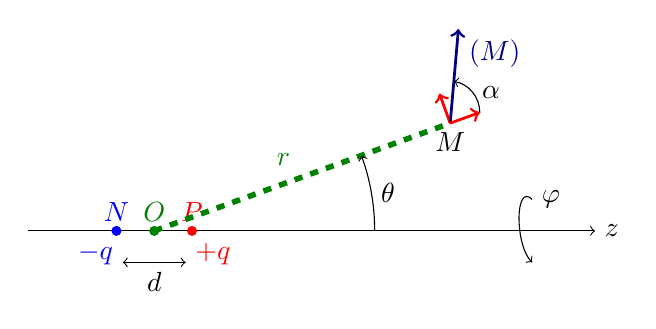
\begin{tikzpicture}[scale=0.4]
\draw[->, black] (-3,0)--(15,0)node[right]{$z$};
    \coordinate (A) at (0,0);
    \coordinate (C) at ({1+ 10 * cos(20)}, {10 * sin(20)});
    \draw[black] (A)++(0,-0.1) node[below left,blue]{$-q$};
    \draw[black] (A)++(-0.2,0) node[above,blue]{$N$};
        \coordinate(B) at (2,0);
     \draw[black] (B)++(0,-0.1) node[below right,red]{$+q$};
     \draw[black] (B)++(0.2,0) node[above,red]{$P$};
    \draw[<->,black] (0,-1) -- node[midway,below] {$d$} (2,-1);
    \filldraw[blue] (A) ++(-0.2,0) circle (4pt);
    \filldraw[green!50!black] (1,0)node[above]{$O$} circle (4pt);
    \filldraw[red] (B) ++(0.2,0) circle (4pt);
    \draw[dashed,line width = 2,green!50!black] (1,0)--node[green!50!black,midway,above left] {$r$} ({1+ 10 * cos(20)}, {10 * sin(20)});
    \draw[black] (C) node[below]{$M$};
       \draw[->, red, line width = 1] (C) -- ++({cos(110)}, {sin(110)})node[left]{$\et$}; 
    \draw[->,black] (8,0) arc[start angle=0, end angle=20, radius=7]node[midway,right]{$\theta$}; % arc de cercle et symbole theta;
    \draw[->, in=135, out=135,black] (13,1)node[right]{$\varphi$} to (13,-1);
     \draw[->, blue!50!black, line width = 1] (C) -- ++({3*cos(85)}, {3*sin(85)})node[below right]{$\E(M)$};
     \draw[->,black] (C) -- ++({cos(20)}, {sin(20)}) arc[start angle=0, end angle=80, radius=1]node[midway,right]{$\alpha$}; % arc de cercle et symbole theta; 
      \draw[->, red, line width = 1] (C) -- ++({cos(20)}, {sin(20)})node[right]{$\er$}; 


     \end{tikzpicture}
  \end{center}
  \begin{align*}
  \tan{\alpha} = \frac{E_{\theta}}{E_{r}} = \frac{\sin\theta}{2\cos\theta} = \frac{1}{2}\tan\theta
  \end{align*}
 \item \eq{\tan\alpha = \frac{1}{2}\tan\theta}
 \eq{\theta = 0 \Lar \alpha =0}
  \eq{\theta = \frac{\pi}{2} \Lar \alpha = \frac{\pi}{2}}
  \eq{\theta = \pi \Lar \alpha = \pi}
  Le champ $\E$ ``tourne'' donc deux fois plus vite que l'axe polaire.
 \item $\vv{p} = qd\( \cos{\theta} \er - \sin{\theta} \et \)$ et $\vv{r} = r\er$
 \eq{\vv{p} \ps \vv{r} = qdr\cos{\theta}}
 \eq{\E(M) = \frac{1}{4\pi \varepsilon_{0}} \ps \frac{3\( \vv{p} \ps \vv{r} \) \vv{r} - \vv{p} r^2}{r^5}}
 \end{enum}
 \end{solu}

\end{exemple}
 
   \begin{theorem}[Expression intrinsèque]
  On peut exprimer $\E$ en fonction de $\vv{p} = qd\( \cos{\theta} \er - \sin{\theta} \et \)$ et $\vv{r} = r\er$ \eq{\E(M) = \frac{1}{4\pi \varepsilon_{0}} \ps \frac{3\( \vv{p} \ps \vv{r} \) \vv{r} - \vv{p} r^2}{r^5}.}
  \end{theorem}
  
  \parag{Topographie} Sur la Fig.~\ref{fig:dip} :
  \begin{liste}
  \item \imp{Equipotentielles} : \begin{liste}
  \item Le plan orthogonal à $(Ox)$ passant par $O$ est l'équipotentielle $V=0$.
  \item Ce plan est un plan d'antisymétrie de la distribution de charge donc le symétrique de l'équipotentielle $V$ par rapport à ce plan est l'équipotentielle $-V$.
  \end{liste}
  \item \imp{Lignes de champ} : \begin{liste}
  \item Orthogonales aux equipotentielles
  \item Pour obtenir une expression exactes des lignes de champs, il faut utiliser l'expression \eq{\E \pv \dl = 0.}
  \item De loin, on pourrait croire que les lignes de champ sont fermées, mais lorsque l'on zoom sur le dipôle, l'approximation dipolaire n'est plus vérifiée et on retrouve le fait que les charge positives et négatives sont respectivement des points de divergence et de convergence des lignes de champ.
  \end{liste}
  \end{liste}
  
\begin{figure}[h!]
\centering
\includegraphics[height=0.5\textwidth]{qneg_equi.pdf}
\caption{Cartes de champ dans un plan $(x,y)$ pour un dipôle électrostatique. L'origine $O$ du repère est pris entre les deux charge et l'axe $y$ est verticale.}
\label{fig:dip}
\end{figure}
%%%%%%%%%%%%%%%%%%%%%%%%

\subsection{Dipôle électrostatique placé dans un champ électrostatique extérieur}

\parag{Action d'un champ uniforme} Considérons un dipôle $\vv{p}$ à l'intérieur d'un champ $\E_{0}$ uniforme.

\begin{center}
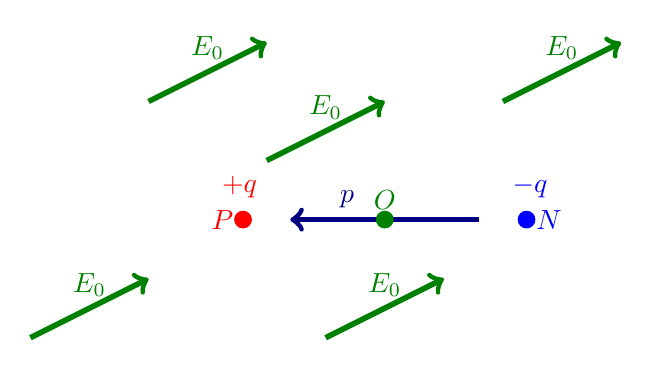
\begin{tikzpicture}[scale=1.5]
    \coordinate (A) at (0,0);
    \draw (A)++(0,0.1) node[above left,red]{$+q$};
    \draw (A)++(-0.2,0) node[left,red]{$P$};
        \coordinate(B) at (2,0);
     \draw (B)++(0,0.1) node[above right,blue]{$-q$};
     \draw (B)++(0.2,0) node[right,blue]{$N$};
    \draw[<-,blue!50!black,line width = 2] (0.2,0) -- node[pos=0.3,above] {$\vv{p}$} (1.8,0);
    \filldraw[red] (A) ++(-0.2,0) circle (2pt);
    \filldraw[blue] (B) ++(0.2,0) circle (2pt);
     \foreach \x/\y in {0/0.5, -1/1, 2/1, -2/-1, 0.5/-1} {
    \draw[green!50!black,->, line width = 2] (\x,\y) -- ++(1,0.5) node[midway,above] {$\Vec{E}_0$};
  }
   \filldraw[green!50!black] (1,0)node[above]{$O$} circle (2pt);
  \end{tikzpicture}
  \end{center}
  
 \noindent Calculons la force exercée par $\E_{0}$ sur le dipôle. \eq{\vv{F}_{\E_{0} \Ar \vv{p}} = q \E_{0}(P) - q \E_{0}(N) = \vv{0}}
  
  \begin{prop}[Résultante des forces]
  La résultante des forces exercées par un champ électrostatique uniforme sur un dipôle est nulle.
  \end{prop}
  
  \noindent Le moment en $O$ des forces exercées par $\E_{0}$ sur le dipôle est 
  \begin{align*}
  \vv{\mc{M}}_{O}(\vv{F}_{\E_{0} \Ar \vv{p}}) &= \vv{OP} \pv q \E_{0} + \vv{ON} \pv \( -q \E_{0}\) \\
  &= \( \vv{OP} - \vv{ON} \) \pv q \E_{0} \\
  &= q \vv{NP} \pv \E_{0} = \vv{p} \pv \E_{0}
  \end{align*}
  
  \begin{remarque}
  $\vv{\mc{M}}_{O}(\vv{F}_{\E_{0} \Ar \vv{p}})$ est indépendant du point $O$, ce moment de force est donc un \imp{couple}.
  \end{remarque}
  
  \begin{prop}[Couple]
  Un champ électrostatique uniforme $\E_{0}$ exerce sur un dipôle électrostatique un couple \eq{\vv{\Gamma} =  \vv{p} \pv \E_{0}}
  qui tend à aligner le moment dipolaire avec le champ $\E_{0}$.
  \end{prop}
  
   \begin{remarque}
  En effet, $\nv{\Gamma} = \nv{p} \nv{E_{0}} \sin\alpha = 0$ si $\alpha = 0$ \ie si $\vv{p}$ et $\E_{0}$ sont alignés.
  \end{remarque}
  
  Regardons à présent l'\imp{énergie potentielle} d'interaction entre $\E_{0}$ et le $\vv{p}$.
  Rappelons que l'énergie potentielle d'une charge $q$ placée dans un potentiel $V$ est \eq{E_{p}(q) = q V.}
  Pour le dipôle électrostatique $\vv{p}$, 
  \begin{align*}
  E_{p}(\vv{p}) &= q V(P) - q V(N) = q\(V(P) - V(N) \)\\
  &= q \int^{V(P)}_{V(N)} \d V  = - q \int^{P}_{N} \E_{0} \ps \dl = - q \E_{0} \ps \vv{NP}\\
  &= - \vv{p} \ps \E_{0} = - \nv{p} \nv{E_{0}} \cos \alpha
  \end{align*}
  
  \begin{center}
\begin{tikzpicture}
\begin{axis}[
    axis lines = middle,
    x label style={at={(axis description cs:1.1,0.5)},anchor=east},
    y label style={at={(axis description cs:0.5,1.1)},anchor=north},
    xlabel = $\alpha$,
    ylabel = $E_{p}$,
    ymin=-1.1, ymax=1.1,
    xmin=-3.5, xmax=3.5,
    xtick=\empty, ytick=\empty, % supprime les graduations
    color=black
]

\addplot [
    domain=-3.5:3.5, 
    samples=100, 
    color=red,
    line width = 2
]
{-cos(deg(x))};


\begin{scope}[on background layer]
    \draw[dashed, red, line width = 1] (axis cs:pi,0)node[below]{$\pi$}--(axis cs:pi,1)--(axis cs:-pi,1)--(axis cs:-pi,0)node[below]{$-\pi$};
    \draw[red] (axis cs:0,1) node[below right]{$\nv{p} \nv{E_{0}}$};
    \draw[red] (axis cs:0,-1) node[below right]{$-\nv{p} \nv{E_{0}}$};
\end{scope}
\begin{scope}[overlay]
    \fill[fill=red] (axis cs:0,1) circle (3pt);
    \fill[fill=red] (axis cs:0,-1) circle (3pt);
\end{scope}
\end{axis}
\end{tikzpicture}
\end{center}

\begin{remarque}
On retrouve le fait que la position $\alpha =0$ corresponde à une position d'équilibre, c'est à dire à un extremum d'énergie potentielle. On peut de plus montrer que cette position d'équilibre est stable alors que la position $\alpha = \pi$ correspond à une position d'équilibre instable.
\end{remarque}

\parag{Action d'un champ non uniforme} Considérons un dipôle $\vv{p}$ à l'intérieur d'un champ $\E$ non uniforme.

\begin{center}
\begin{tikzpicture}[scale=1.5]
    \coordinate (A) at (0,0);
    \draw (A)++(0,0.1) node[above left,red]{$+q$};
    \draw (A)++(-0.2,0) node[left,red]{$P$};
        \coordinate(B) at (2,0);
     \draw (B)++(0,0.1) node[above right,blue]{$-q$};
     \draw (B)++(0.2,0) node[right,blue]{$N$};
    \draw[<-,blue!50!black,line width = 2] (0.2,0) -- node[midway,above] {$\vv{p}$} (1.8,0);
    
    
    % Les deux courbes
    \coordinate (C) at (3.5,2.3);
    \coordinate (D) at (2.5,1.8);
     \coordinate (CP) at (3.8,2.2);
    \coordinate (FN) at (4,1.7);
    \coordinate (E) at (-3,-1);
    \coordinate (F) at (4,1.3);
    \coordinate (G) at (3,1);
    \coordinate (H) at (3,-1);
    \coordinate (P) at (-0.2,0);
    \coordinate (N) at (2.2,0);
    \coordinate (EP) at (-1.2,-1);
    \coordinate (HN) at (1.2,-1);
    \coordinate (DP) at (2.5,1.6);
    \coordinate (GN) at (2.8,1);
    
    \draw[postaction={decorate,decoration={markings, mark=at position 0.5 with {\arrow{>}}}}, green!50!black, line width=1.5] (C) to[out=-90,in=-10] (D) to[out=170,in=45] (E);
    \draw[postaction={decorate,decoration={markings, mark=at position 0.5 with {\arrow{>}}}}, green!50!black, line width=1.5] (F) to[out=135,in=90] (G) to[out=-90,in=45] (H);
     \draw[postaction={decorate,decoration={markings, mark=at position 0.5 with {\arrow{>}}}}, green!50!black, line width=1.5] (CP) to[out=-120,in=-10] (DP) to[out=170,in=45] (P) to[out=-135,in=45] (EP);
    \draw[postaction={decorate,decoration={markings, mark=at position 0.5 with {\arrow{>}}}}, green!50!black, line width=1.5] (FN) to[out=180,in=90] (GN) to[out=-90,in=45] (N) to[out=-135,in=45]  (HN);
    \draw (-1, 1) node[left, green!50!black]{$\E$};
    \filldraw[red] (A) ++(-0.2,0) circle (2pt);
    \filldraw[blue] (B) ++(0.2,0) circle (2pt);
  \end{tikzpicture}
  \end{center}

Dans l'approximation dipolaire, les variations de $\E(M)$ sont faibles entre $P$ et $N$ de sorte que 
\eq{\E(P) = \E(O) + \delta \E(P) \quad \quad \textnormal{avec} \quad \quad \lVert\delta \E(P)\rVert \ll \lVert \E(O)\rVert }
\eq{\E(N) = \E(O) + \delta \E(N) \quad \quad \textnormal{avec} \quad \quad \lVert\delta \E(N)\rVert \ll \lVert \E(O)\rVert }


Le moment des forces exercées par $\E(M)$ sur le dipôle est donc
\begin{align*}
  \vv{\mc{M}}_{O}(\vv{F}_{\E \Ar \vv{p}}) &= \vv{OP} \pv q \( \E(O) + \delta \E(P)\)  -\vv{ON} \pv q\( \E(O) + \delta \E(N)\) \\
  &= q \vv{NP} \pv \E_{0} = \vv{p} \pv \E(O) + q \vv{OP} \pv \delta \E(P) - q \vv{ON} \pv \delta \E(N)\\
  &\simeq \vv{p} \pv \E(O).
  \end{align*}
  
  \begin{prop}
  Un champ électrostatique non uniforme $\E$ exerce sur un dipôle électrostatique un moment qui tend à aligner le dipôle avec la ligne de champ qui passe en son centre.
  \eq{\vv{\mc{M}}_{O}(\vv{F}_{\E \Ar \vv{p}}) \simeq \vv{p} \pv \E(O)}
  \end{prop}
  
 
  
  \begin{center}
\begin{tikzpicture}[scale=1.5]
    \coordinate (A) at (0,-1);
    \draw (A)++(0.1,0.1) node[above left,red]{$+q$};
    \draw (A)++(-0.4,0) node[left,red]{$P$};
        \coordinate(B) at (1.5,0.5);
     \draw (B)++(-0,0.1) node[above left,blue]{$-q$};
     \draw (B)++(0.2,0) node[right,blue]{$N$};
    \draw[<-,blue!50!black,line width = 2] (0.25, -0.75) -- node[midway,above] {$\vv{p}$} (1.25,0.25);
    
    
    % Les deux courbes
    \coordinate (C) at (3.5,2.3);
    \coordinate (D) at (2.5,1.8);
     \coordinate (CP) at (3.8,2.2);
    \coordinate (FN) at (4,1.7);
    \coordinate (E) at (-3,-1);
    \coordinate (F) at (4,1.3);
    \coordinate (G) at (3,1);
    \coordinate (H) at (3,-1);
    \coordinate (P) at (-0.2,0);
    \coordinate (N) at (2.2,0);
    \coordinate (EP) at (-1.2,-1);
    \coordinate (HN) at (1.2,-1);
    \coordinate (DP) at (2.5,1.6);
    \coordinate (GN) at (2.8,1);
    
    \draw[postaction={decorate,decoration={markings, mark=at position 0.6 with {\arrow{>}}}}, green!50!black, line width=1.5] (C) to[out=-90,in=-10] (D) to[out=170,in=45] (E);
    \draw[postaction={decorate,decoration={markings, mark=at position 0.6 with {\arrow{>}}}}, green!50!black, line width=1.5] (F) to[out=135,in=90] (G) to[out=-90,in=45] (H);
     \draw[postaction={decorate,decoration={markings, mark=at position 0.6 with {\arrow{>}}}}, green!50!black, line width=1.5] (CP) to[out=-120,in=-10] (DP) to[out=170,in=45] (P) to[out=-135,in=45] (EP);
    \draw[postaction={decorate,decoration={markings, mark=at position 0.6 with {\arrow{>}}}}, green!50!black, line width=1.5] (FN) to[out=180,in=90] (GN) to[out=-90,in=45] (N) to[out=-135,in=45]  (HN);
    \draw (-1, 1) node[left, green!50!black]{$\E$};
   
     \draw[->,red!50!black,line width = 2] (B) --  ++(0.75,0.75) node[left=0.1] {$-q\E(N)$};
      \draw[->,red!50!black,line width = 2] (A) --  ++(-0.5,-0.5) node[right=0.1] {$+q\E(N)$};
      
      \filldraw[red] (A) ++(0,0) circle (2pt);
    \filldraw[blue] (B) ++(0,0) circle (2pt);
    
  \end{tikzpicture}
  \end{center}
  
  \noindent Qualitativement, supposons que le dipôle s'est aligné avec la ligne de champ passant en son centre. Ici $\lVert \E(N)\rVert > \lVert \E(P)\rVert $. Le dipôle va donc être entrainer vers la zone de champ fort. 
  
  \noindent Quantitativement, \begin{align*} 
  \vv{F}_{\E \Ar \vv{p}} &= q \( \E(O) + \delta \E(P)\)  - q\( \E(O) + \delta \E(N)\)  \\
  &= q \( \delta \E(P) -  \delta \E(N)\) 
  \end{align*}
  En faisant un \acl{DL} à l'ordre 1 pour \eq{\vv{NP} = \Delta x \ps \ex + \Delta y \ps \ey + \Delta z  \ps\ez} 
  \eq{ \delta E_{i \in \{x,y,z \}}(P) = \frac{\Delta x}{2} \ps \dr{E_{i}(O)}{x}+ \frac{\Delta y}{2} \ps \dr{E_{i}(O)}{y} + \frac{\Delta z}{2} \ps \dr{E_{i}(O)}{z}}
  \eq{ \delta E_{i \in \{x,y,z \}}(N) = -\frac{\Delta x}{2} \ps \dr{E_{i}(O)}{x} - \frac{\Delta y}{2} \ps \dr{E_{i}(O)}{y} - \frac{\Delta z}{2} \ps \dr{E_{i}(O)}{z} = - \delta E_{i}(P) }
  \begin{align*} 
  \vv{F_{i}}_{\E \Ar \vv{p}} = \vv{F}_{\E \Ar \vv{p}} \ps \vv{e}_{i} &= q  \( \Delta x\ps \dr{E_{i}(O)}{x}+ \Delta y \ps \dr{E_{i}(O)}{y} + \Delta z \ps \dr{E_{i}(O)}{z} \) = \(\vv{p} \ps \Grad{} \)E_{i}
  \end{align*}
  on obtient \eq{ \vv{F}_{\E \Ar \vv{p}} = \(\vv{p} \ps \Grad{} \) \E.}
 
 \begin{theorem}
  La résultante des forces exercées par un champ électrostatique $\E$ sur un dipôle $\vv{p}$ est dans le cas général \eq{ \vv{F}_{\E \Ar \vv{p}} = \(\vv{p} \ps \Grad{} \) \E.}
 \end{theorem}
 
 \begin{remarque}
 Pour un champ uniforme, on retrouve 
 \eq{ \vv{F}_{\E_{0} \Ar \vv{p}} = \vv{0}.}

 \end{remarque}
  
  \begin{prop}
  Un champ électrostatique non uniforme exerce sur un dipôle électrostatique une force qui tend à attirer le dipôle vers les zones de champ fort.
  \end{prop}
  
  
  
  






\end{document}
